
% *** Authors should verify (and, if needed, correct) their LaTeX system  ***
% *** with the testflow diagnostic prior to trusting their LaTeX platform ***
% *** with production work. The IEEE's font choices and paper sizes can   ***
% *** trigger bugs that do not appear when using other class files.       ***                          ***
% The testflow support page is at:
% http://www.michaelshell.org/tex/testflow/



\documentclass[journal,letterpaper]{IEEEtran}
%
% If IEEEtran.cls has not been installed into the LaTeX system files,
% manually specify the path to it like:
% \documentclass[journal]{../sty/IEEEtran}


% *** CITATION PACKAGES ***
%
\usepackage{cite}
\usepackage{lipsum}
\usepackage{multirow,hhline}
\usepackage{booktabs,xcolor,siunitx,colortbl} %color cells
\usepackage{makecell}  %bold lines
\usepackage{units}  %nice fraction
\usepackage[numbered]{mcode}
\usepackage{amsmath,amssymb,latexsym,float,epsfig}
\usepackage{upgreek,mathtools}
%\usepackage{flushend}
\usepackage{slashbox}
\usepackage{comment}
\usepackage{listings}
%the subcaption package overwrites the caption size, so you need the follow-on command
\usepackage{subcaption}
\usepackage{caption}

\usepackage{graphicx}
%\usepackage{array}
%\usepackage{hhline} 
%\usepackage[math]{cellspace}
%\newcommand{\degree}{\ensuremath{^\circ}}
%\cellspacetoplimit 2pt
%\cellspacebottomlimit 2pt
%\usepackage{colortbl}
%\newcolumntype{C}{c<{\kern\tabcolsep}@{}}

\DeclareCaptionFormat{mycaptionfont}{\fontsize{8}{7}\selectfont#1#2#3}
\captionsetup{format=mycaptionfont}

\definecolor{TableBackgroundColor}{HTML}{FFFFFF}
\definecolor{white}{HTML}{FFFFFF}
\definecolor{red}{HTML}{FF0000}
\definecolor{black}{HTML}{000000}
\definecolor{lightpink}{HTML}{F2DCDB}
\definecolor{lightblue}{HTML}{DAEEF3}
\definecolor{lightpurple}{HTML}{E4DFEC}
\definecolor{lightyellow}{HTML}{FFFFAE}
\definecolor{lightgray}{HTML}{EFEFEF}
\definecolor{nearwhite}{HTML}{FEFEFE}

%\newcommand{\UC}[1]{\colorbox{yellow}{#1}}  %U color
\newcommand{\reducedstrut}{\vrule width 0pt height .9\ht\strutbox depth .9\dp\strutbox\relax}
\newcommand{\UC}[1]{%
  \begingroup
  \setlength{\fboxsep}{0pt}%  
  \colorbox{lightpink}{\reducedstrut#1\/}%
  \endgroup
}
\newcommand{\UW}[1]{%
  \begingroup
  \setlength{\fboxsep}{0pt}%  
  \colorbox{lightblue}{\reducedstrut#1\/}%
  \endgroup
}

\newcommand{\UV}[1]{%
  \begingroup
  \setlength{\fboxsep}{0pt}%  
  \colorbox{lightpurple}{\reducedstrut#1\/}%
  \endgroup
}

\newcommand{\thickhline}{%
    \noalign {\ifnum 0=`}\fi \hrule height 1pt
    \futurelet \reserved@a \@xhline
}
\newcolumntype{?}{!{\vrule width 1pt}}

%\ifCLASSOPTIONcaptionsoff
%  \usepackage[nomarkers]{endfloat}
% \let\MYoriglatexcaption\caption
% \renewcommand{\caption}[2][\relax]{\MYoriglatexcaption[#2]{#2}}
%\fi
% endfloat.sty was written by James Darrell McCauley, Jeff Goldberg and 
% Axel Sommerfeldt. This package may be useful when used in conjunction with 
% IEEEtran.cls'  captionsoff option. Some IEEE journals/societies require that
% submissions have lists of figures/tables at the end of the paper and that
% figures/tables without any captions are placed on a page by themselves at
% the end of the document. If needed, the draftcls IEEEtran class option or
% \CLASSINPUTbaselinestretch interface can be used to increase the line
% spacing as well. Be sure and use the nomarkers option of endfloat to
% prevent endfloat from "marking" where the figures would have been placed
% in the text. The two hack lines of code above are a slight modification of
% that suggested by in the endfloat docs (section 8.4.1) to ensure that
% the full captions always appear in the list of figures/tables - even if
% the user used the short optional argument of \caption[]{}.
% IEEE papers do not typically make use of \caption[]'s optional argument,
% so this should not be an issue. A similar trick can be used to disable
% captions of packages such as subfig.sty that lack options to turn off
% the subcaptions:
% For subfig.sty:
% \let\MYorigsubfloat\subfloat
% \renewcommand{\subfloat}[2][\relax]{\MYorigsubfloat[]{#2}}
% However, the above trick will not work if both optional arguments of
% the \subfloat command are used. Furthermore, there needs to be a
% description of each subfigure *somewhere* and endfloat does not add
% subfigure captions to its list of figures. Thus, the best approach is to
% avoid the use of subfigure captions (many IEEE journals avoid them anyway)
% and instead reference/explain all the subfigures within the main caption.
% The latest version of endfloat.sty and its documentation can obtained at:
% http://www.ctan.org/pkg/endfloat
%
% The IEEEtran \ifCLASSOPTIONcaptionsoff conditional can also be used
% later in the document, say, to conditionally put the References on a 
% page by themselves.




% *** PDF, URL AND HYPERLINK PACKAGES ***
%
%\usepackage{url}
% url.sty was written by Donald Arseneau. It provides better support for
% handling and breaking URLs. url.sty is already installed on most LaTeX
% systems. The latest version and documentation can be obtained at:
% http://www.ctan.org/pkg/url
% Basically, \url{my_url_here}.




% *** Do not adjust lengths that control margins, column widths, etc. ***
% *** Do not use packages that alter fonts (such as pslatex).         ***
% There should be no need to do such things with IEEEtran.cls V1.6 and later.
% (Unless specifically asked to do so by the journal or conference you plan
% to submit to, of course. )


% correct bad hyphenation here
\hyphenation{op-tical net-works semi-conduc-tor}


\begin{document}
\bstctlcite{IEEEexample:BSTcontrol}
%
% paper title
% Titles are generally capitalized except for words such as a, an, and, as,
% at, but, by, for, in, nor, of, on, or, the, to and up, which are usually
% not capitalized unless they are the first or last word of the title.
% Linebreaks \\ can be used within to get better formatting as desired.
% Do not put math or special symbols in the title.
\title{A reference implementation of the AES S-Box}
%
%
% author names and IEEE memberships
% note positions of commas and nonbreaking spaces ( ~ ) LaTeX will not break
% a structure at a ~ so this keeps an author's name from being broken across
% two lines.
% use \thanks{} to gain access to the first footnote area
% a separate \thanks must be used for each paragraph as LaTeX2e's \thanks
% was not built to handle multiple paragraphs
%

\author{{Brian~Degnan, and~Gregory~Durgin}% <-this % stops a space
\thanks{B. Degnan (https://orcid.org/0000-0002-6567-6998) and G. Durgin are with the Department
of Electrical and Computer Engineering, Georgia Institute of Technology, Atlanta,
GA, 30332 USA e-mail: (see http://www.propagation.gatech.edu/).}% <-this % stops a space
%\thanks{Others are with Anonymous University.}% <-this % stops a space
\thanks{This document was compiled on \today.}}
% note the % following the last \IEEEmembership and also \thanks - 
% these prevent an unwanted space from occurring between the last author name
% and the end of the author line. i.e., if you had this:
% 
% \author{....lastname \thanks{...} \thanks{...} }
%                     ^------------^------------^----Do not want these spaces!
%
% a space would be appended to the last name and could cause every name on that
% line to be shifted left slightly. This is one of those "LaTeX things". For
% instance, "\textbf{A} \textbf{B}" will typeset as "A B" not "AB". To get
% "AB" then you have to do: "\textbf{A}\textbf{B}"
% \thanks is no different in this regard, so shield the last } of each \thanks
% that ends a line with a % and do not let a space in before the next \thanks.
% Spaces after \IEEEmembership other than the last one are OK (and needed) as
% you are supposed to have spaces between the names. For what it is worth,
% this is a minor point as most people would not even notice if the said evil
% space somehow managed to creep in.



% The paper headers

%\markboth{Journal of \LaTeX\ Class Files,~Vol.~14, No.~8, August~2015}%
%{Shell \MakeLowercase{\textit{et al.}}: Bare Demo of IEEEtran.cls for IEEE Journals}

% The only time the second header will appear is for the odd numbered pages
% after the title page when using the twoside option.
% 
% *** Note that you probably will NOT want to include the author's ***
% *** name in the headers of peer review papers.                   ***
% You can use \ifCLASSOPTIONpeerreview for conditional compilation here if
% you desire.




% If you want to put a publisher's ID mark on the page you can do it like
% this:
%\IEEEpubid{0000--0000/00\$00.00~\copyright~2015 IEEE}
% Remember, if you use this you must call \IEEEpubidadjcol in the second
% column for its text to clear the IEEEpubid mark.



% use for special paper notices
%\IEEEspecialpapernotice{(Invited Paper)}




% make the title area
\maketitle

% As a general rule, do not put math, special symbols or citations
% in the abstract or keywords.
\begin{abstract}
The Advanced Encryption Standard (AES) is a specification for the encryption of electronic data.  The substitution-permutation network architecture of AES uses the irreducible polynomial of  \(x^8+x^4+x^3+x+1\) that provides a non-linear permutations for the cipher.  In this work, we describe the complete circuits and reductions required to implement a non-lookup table based S-Box in hardware for the AES irreducible polynomial in order to create a reference for comparisons.  The verification script is written in the BASH shell so that they can be easily modified for integration to different simulation and verification tools. \end{abstract}

% Note that keywords are not normally used for peerreview papers.
\begin{IEEEkeywords}
AES, block cipher, simulation, RFID, IoT
\end{IEEEkeywords}

\section*{Motivation}
The Advanced Encryption Standard (AES) is a block cipher based on a substitution-permutation network\cite{fips197}.  Although the AES cipher has been approved for over 20 years, we were unable to find a hardware implementation reference that was suitable for comparisons against lightweight ciphers. This document attempts a minimal ``nothing up the sleeves'' transistor implementation of the non-linear component of AES, the S-Box.  This work attempts to be the concisely written culmination of many other AES implementations.  There is very little, if any, novel content in this document; however, as we were unable to explicitly find the information required for a research, and this document was created.  Our focus of research includes power constrained devices, and the bulk of AES implementations use lookup tables for the Galois Field logic substitutions, or do not clearly explain the circuit implementation\cite{rudra2001efficient,wang2014application,gueron2016hardware}.  This work attempts to be a complete description and verification for AES targeting a custom semiconductor implementation that does not use lookup tables.  The work is based off of the optimized S-Box by the AES authors \cite{rijmen2000efficient} combined with an approach alluded to by Satoh et al \cite{satoh2001compact}.  This work extends previous work by complete mathematical descriptions, circuit logic implementations, and logic verification scripts.

\section{AES}
The AES algorithm is a block cipher that uses a 128, 192, or 256 bit keys to operation on a block of 128 bits of data.  The shorthand notation for these configurations are AES128/128, AES128/192 and AES128/256 and the algorithm uses \(n\) rounds that are 10, 12, and 14 respectively.  The AES algorithm is not the focus of this work, but the S-Box that underpins the non-linearity that is used in the cipher, which is the irreducible polynomial of \(x^8+x^4+x^3+x+1\).

\subsection{Review GF(2) Polynomials}
As a review of GF(2) polynomials used in this work, GF(2) polynomials represent rings of numbers.  As an example, the mapping of coefficients to numbers for \(x^2+x+1\) is given by the following table:
\begin{center}
\begin{tabular}{|r|c|r|}
\hline
dec & bin & polynomial \\
\hline
0 & 000 & \(0\) \\
1 & 001 & \(1\) \\
2 & 010 & \(x\) \\
3 & 011 & \(x+1\) \\
4 & 100 & \(x^2\) \\
5 & 101 & \(x^2+1\) \\
6 & 110 & \(x^2+x\) \\
7 & 111 & \(x^2+x+1\) \\
\hline
\end{tabular}
\end{center}

AES uses the same irreducible polynomial for every operation, which is \(x^8+x^4+x^3+x+1\).  This polynomial results in 9-bits, and is 0x11B in hexadecimal, or 100011011 in binary.  You will notice that the 9-bits results in one bit more than you have in an 8-bit byte, and this allows the modulus to be the XOR of 0x1b.  

\subsection{Special Properties of GF(2) Polynomials}
The logic reductions used in this work are based GF(2) polynomials.  The computations on \(GF(2^8)\) are done by reducing the field to a lower order composite fields of
\begin{align}
\label{eqn:GFdecomposition}
GF(2^2)&\rightarrow GF(2)&:x^2+x+1\nonumber \\ 
GF((2^2)^2)&\rightarrow GF(2^2)&:x^2+x+\varphi\\
GF(((2^2)^2)^2)&\rightarrow GF((2^2)^2)&:x^2+x+\lambda \nonumber
\end{align}
where \(\varphi=\{10\}_2\) and \(\lambda=\{1100\}_2\).  As previously stated, \(GF(2^2)\) polynomials can be decomposed to lower-order composite fields where \(n_1x+n_0\).  Therefore, and binary number, \(k\), can be split into \(k_Hx+k_L\).  As an example, for \(k=\{1001\}_2\), the value \(k\) is \(k_Hx+k_L\), resulting in 
\(\{10\}_2x+\{01\}_2\), which can be further reduced to \(\{1\}_2x+\{0\}_2\) and \(\{0\}_2x+\{1\}_2\) as high and low terms.


\section{aesbash.sh}
In order to facilitate the simulation and representation of hardware that is described in this document, 
the AES S-Box has been implemented as a virtual logic implementation through the aesbash.sh script\cite{degnan:github:aesbash}.  The functions in the script are bitwise, and represent the circuit architectures described in Section \ref{sec:sbox}.   The script was designed and used under BASH version 3.2.57.  The functions are described in Table \ref{tab:aesbash} and are internally constructed as logic would be in a hardware implementation.  For this reason, a multiply of two, 4-bit words is implemented as a single 8-bit input because this format is easily transcribed to SPICE modeling conventions.  The archive, \cite{degnan:github:aesbash}, also contain test and verification scripts that generate all of the tables in this work.

\begin{table}[h]
 \caption{Script functions that emulate hardware blocks}
  \label{tab:aesbash}
\centering
\begin{tabular}{|@{\hskip3pt}l@{\hskip3pt}|@{\hskip3pt}c@{\hskip3pt}|@{\hskip3pt}c@{\hskip3pt}|@{\hskip3pt}l@{\hskip3pt}|}
\hline
 &  & bit & \\
function & args & width & description\\
\hline
 aes\_affine & 1 & 8 & calculate affine transform\\ \hline
 aes\_affineinv & 1 & 8 & inverse affine transform\\ \hline
 aes\_invGF24 & 1 & 4 & multiplicative inverse of input \\ \hline
 aes\_isomorphic & 1 & 8 & isomorphic transform\\ \hline
 aes\_isomorphicinv & 1 & 8 & inverse isomorphic transform\\ \hline
 aes\_lambdamultiply & 1 & 4 & multiplication by \(\lambda=\{1100\}\) \\ \hline
 aes\_multGF2 & 1 & 4 & mult. of 2, 2-bit numbers \\ \hline
 aes\_multGF24 & 1 & 8 & mult. of 2, 4-bit numbers\\ \hline
 aes\_multiplicativeinversion & 1 & 8 & multiplicative inversion\\ \hline
 aes\_phimultiply & 1 & 2 & mult. by constant \(\varphi=\{10\}\) \\ \hline
 aes\_squarerGF24 & 1 & 4 & the square of the input \\ \hline
 aes\_subbyte & 1 & 8 & subbyte calculation\\ \hline
 aes\_subbyteinv & 1 & 8 & inverse subbyte calculation\\ \hline
 aesbash\_verdep & 0 & 0 & check and download deps.\\ \hline
 helplatex & 0 & 0 & autogenerate this table\\ \hline
\end{tabular}
\end{table}


\section{S-Box construction}
\label{sec:sbox}
The AES S-Box is based on a non-linear boolean function that replaces an element of a finite field with its modular multiplicative inverse. Thus, \(x \rightarrow x^{-1}\), where \(x\) represents an element of the finite field and \(x^{-1}\) denotes its multiplicative inverse in the field.  As the S-Box is invertible, there are two modes of operation, Subbyte and InvSubbyte.  In the Subbyte case, the data is run through a multiplicative inversion and then an affine transform.  To invert the result, the data is run through an affine transform inversion, and then the same multiplicative inversion mathematics as the Subbyte.   The software approach to inverse fields is often to use a lookup table, which is not necessarily the best implementation in hardware.  An efficient hardware construction for calculating the multiplicative inverse in \(GF\left(2^8\right)\) was given by Rijmen in \cite{rijmen2000efficient}, and this work was improved upon by Satoh et al. in \cite{satoh2001compact}.  The work described here is a complete implementation of the work in \cite{satoh2001compact} with explanations and verification scripts. 

\begin{figure}[t]
\centering
\begin{tabular}{@{}c@{}}
\subcaptionbox{\label{fig:aes-subbyte}}{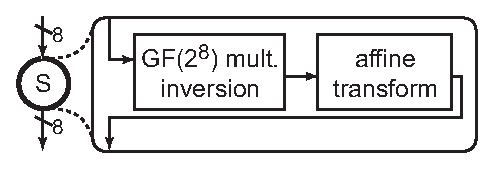
\includegraphics[width=2.8in]{eps/aes-subbyte.eps}}  \\
\\
\subcaptionbox{\label{fig:aes-invsubbyte}}{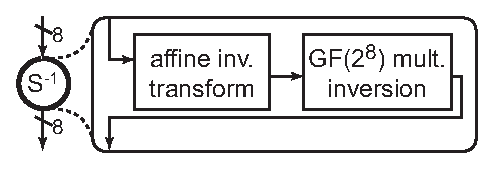
\includegraphics[width=2.8in]{eps/aes-invsubbyte.eps}} \\
\end{tabular}
\label{fig:hasharch}
\caption{An illustration of the S-Box architecture is presented.  (a) is the Subbyte calculation used in encryption that consists of a multiplicative inversion to an affine transform.  (b) is the InvSubbyte calculation used in decryption that consists of an inverse affine transform to the multiplicative inversion module. }
\end{figure}

\subsection{SubByte}
The SubByte is computed by calculating the Multiplicative Inversion in \(GF(2^8)\), described in Section \ref{sec:multiplicativeinversionmodule},  and then an affine transformation, \(Af\), described in Section \ref{sec:affinetransform}, where an 8-bit input becomes an 8-bit output that is then passed to the multiplicative inversion module.  

\begin{table}[h]
 \caption{The pre-calculated byte substitution. }
  \label{tab:subbyte}
\centering
%autogenerated by aestest_subbytetable via aestest_subbytetable.sh
\begin{tabular}{@{\hskip3pt}c@{\hskip3pt}|@{\hskip3pt}c@{\hskip3pt}|@{\hskip3pt}c@{\hskip3pt}|@{\hskip3pt}c@{\hskip3pt}|@{\hskip3pt}c@{\hskip3pt}|@{\hskip3pt}c@{\hskip3pt}|@{\hskip3pt}c@{\hskip3pt}|@{\hskip3pt}c@{\hskip3pt}|@{\hskip3pt}c@{\hskip3pt}|@{\hskip3pt}c@{\hskip3pt}|@{\hskip3pt}c@{\hskip3pt}|@{\hskip3pt}c@{\hskip3pt}|@{\hskip3pt}c@{\hskip3pt}|@{\hskip3pt}c@{\hskip3pt}|@{\hskip3pt}c@{\hskip3pt}|@{\hskip3pt}c@{\hskip3pt}|@{\hskip3pt}c@{\hskip3pt}|}
 & 00 & 01 & 02 & 03 & 04 & 05 & 06 & 07 & 08 & 09 & 0a & 0b & 0c & 0d & 0e & 0f \\ 
 \hline
00 &63 & 7c & 77 & 7b & f2 & 6b & 6f & c5 & 30 & 01 & 67 & 2b & fe & d7 & ab & 76 \\ 
 \hline
10 &ca & 82 & c9 & 7d & fa & 59 & 47 & f0 & ad & d4 & a2 & af & 9c & a4 & 72 & c0 \\ 
 \hline
20 &b7 & fd & 93 & 26 & 36 & 3f & f7 & cc & 34 & a5 & e5 & f1 & 71 & d8 & 31 & 15 \\ 
 \hline
30 &04 & c7 & 23 & c3 & 18 & 96 & 05 & 9a & 07 & 12 & 80 & e2 & eb & 27 & b2 & 75 \\ 
 \hline
40 &09 & 83 & 2c & 1a & 1b & 6e & 5a & a0 & 52 & 3b & d6 & b3 & 29 & e3 & 2f & 84 \\ 
 \hline
50 &53 & d1 & 00 & ed & 20 & fc & b1 & 5b & 6a & cb & be & 39 & 4a & 4c & 58 & cf \\ 
 \hline
60 &d0 & ef & aa & fb & 43 & 4d & 33 & 85 & 45 & f9 & 02 & 7f & 50 & 3c & 9f & a8 \\ 
 \hline
70 &51 & a3 & 40 & 8f & 92 & 9d & 38 & f5 & bc & b6 & da & 21 & 10 & ff & f3 & d2 \\ 
 \hline
80 &cd & 0c & 13 & ec & 5f & 97 & 44 & 17 & c4 & a7 & 7e & 3d & 64 & 5d & 19 & 73 \\ 
 \hline
90 &60 & 81 & 4f & dc & 22 & 2a & 90 & 88 & 46 & ee & b8 & 14 & de & 5e & 0b & db \\ 
 \hline
a0 &e0 & 32 & 3a & 0a & 49 & 06 & 24 & 5c & c2 & d3 & ac & 62 & 91 & 95 & e4 & 79 \\ 
 \hline
b0 &e7 & c8 & 37 & 6d & 8d & d5 & 4e & a9 & 6c & 56 & f4 & ea & 65 & 7a & ae & 08 \\ 
 \hline
c0 &ba & 78 & 25 & 2e & 1c & a6 & b4 & c6 & e8 & dd & 74 & 1f & 4b & bd & 8b & 8a \\ 
 \hline
d0 &70 & 3e & b5 & 66 & 48 & 03 & f6 & 0e & 61 & 35 & 57 & b9 & 86 & c1 & 1d & 9e \\ 
 \hline
e0 &e1 & f8 & 98 & 11 & 69 & d9 & 8e & 94 & 9b & 1e & 87 & e9 & ce & 55 & 28 & df \\ 
 \hline
f0 &8c & a1 & 89 & 0d & bf & e6 & 42 & 68 & 41 & 99 & 2d & 0f & b0 & 54 & bb & 16 \\ 
 \hline
\end{tabular}
\end{table}
The pre-calculated values for the SubByte function are reported in Table \ref{tab:subbyte}, and this output was automatically generated by the script   {aestest\_subbytetable.sh}, which iterates through every input.  A single input can be evaluated by 
\begin{lstlisting}[language=bash]
#!/bin/sh
source aesbash.sh
aes_subbyte "00100000"
\end{lstlisting}
where ``00100000" is the function input, resulting in the output of ``10110111".


\subsection{Affine Transformation}
\label{sec:affinetransform}
The affine transform is defined by:

\begin{align}
\label{eqn:aff}
Af(a) = \left(
 \begin{array}{@{\hskip2pt}c@{\hskip2pt}@{\hskip2pt}c@{\hskip2pt}@{\hskip2pt}c@{\hskip2pt}@{\hskip2pt}c@{\hskip2pt}@{\hskip2pt}c@{\hskip2pt}@{\hskip2pt}c@{\hskip2pt}@{\hskip2pt}c@{\hskip2pt}@{\hskip2pt}c@{\hskip2pt}}
  1 & 1 & 1 & 1 & 1 & 0 & 0 & 0 \\
  0 & 1 & 1 & 1 & 1 & 1 & 0 & 0 \\
  0 & 0 & 1 & 1 & 1 & 1 & 1 & 0 \\
  0 & 0 & 0 & 1 & 1 & 1 & 1 & 1 \\
  1 & 0 & 0 & 0 & 1 & 1 & 1 & 1 \\
  1 & 1 & 0 & 0 & 0 & 1 & 1 & 1 \\
  1 & 1 & 1 & 0 & 0 & 0 & 1 & 1 \\
  1 & 1 & 1 & 1 & 0 & 0 & 0 & 1
 \end{array}
 \right)
 \times
 \begin{pmatrix}
  a_7 \\
  a_6 \\
  a_5 \\
  a_4 \\
  a_3 \\
  a_2 \\
  a_1 \\
  a_0 
 \end{pmatrix}
 \oplus
  \begin{pmatrix}
  0 \\
  1 \\
  1 \\
  0 \\
  0 \\
  0 \\
  1 \\
  1 
 \end{pmatrix}
\end{align}

In equation (\ref{eqn:aff}), the input bit \(a_x\) is mapped to the affine transform.  This results in
\begin{alignat}{3}
\label{matrix:affine}
Af(a)&=
 \begin{pmatrix}
  af_7 \\
  af_6 \\
  af_5 \\
  af_4 \\
  af_3 \\
  af_2 \\
  af_1 \\
  af_0 
 \end{pmatrix}
  &=
  \begin{pmatrix}
  \multicolumn{8}{c}{a_7 \oplus a_6 \oplus a_5 \oplus a_4 \oplus a_3 \oplus 0} \\
  \multicolumn{8}{c}{a_6 \oplus a_5 \oplus a_4 \oplus a_3 \oplus a_2 \oplus 1} \\
  \multicolumn{8}{c}{a_5 \oplus a_4 \oplus a_3 \oplus a_2 \oplus a_1 \oplus 1} \\
  \multicolumn{8}{c}{a_4 \oplus a_3 \oplus a_2 \oplus a_1 \oplus a_0 \oplus 0} \\
  \multicolumn{8}{c}{a_7 \oplus a_3 \oplus a_2 \oplus a_1 \oplus a_0 \oplus 0} \\
  \multicolumn{8}{c}{a_7 \oplus a_6 \oplus a_2 \oplus a_1 \oplus a_0 \oplus 0} \\
  \multicolumn{8}{c}{a_7 \oplus a_6 \oplus a_5 \oplus a_1 \oplus a_0 \oplus 1} \\
  \multicolumn{8}{c}{a_7 \oplus a_6 \oplus a_5 \oplus a_4 \oplus a_0 \oplus 1} \\
 \end{pmatrix},
\end{alignat}
where each ``1'' in the transform field corresponds to an XOR, which results in the logic shown in equation (\ref{matrix:affine}).


\begin{table}[t]
 \caption{The pre-calculated affine transform logic results. }
  \label{tab:aesaffinetransform}
\centering
%autogenerated by aestest_affine via aestest_affine.sh
\begin{tabular}{@{\hskip3pt}c@{\hskip3pt}|@{\hskip3pt}c@{\hskip3pt}|@{\hskip3pt}c@{\hskip3pt}|@{\hskip3pt}c@{\hskip3pt}|@{\hskip3pt}c@{\hskip3pt}|@{\hskip3pt}c@{\hskip3pt}|@{\hskip3pt}c@{\hskip3pt}|@{\hskip3pt}c@{\hskip3pt}|@{\hskip3pt}c@{\hskip3pt}|@{\hskip3pt}c@{\hskip3pt}|@{\hskip3pt}c@{\hskip3pt}|@{\hskip3pt}c@{\hskip3pt}|@{\hskip3pt}c@{\hskip3pt}|@{\hskip3pt}c@{\hskip3pt}|@{\hskip3pt}c@{\hskip3pt}|@{\hskip3pt}c@{\hskip3pt}|@{\hskip3pt}c@{\hskip3pt}|}
 & 00 & 01 & 02 & 03 & 04 & 05 & 06 & 07 & 08 & 09 & 0a & 0b & 0c & 0d & 0e & 0f \\ 
 \hline
00 &63 & 7c & 5d & 42 & 1f & 00 & 21 & 3e & 9b & 84 & a5 & ba & e7 & f8 & d9 & c6 \\ 
 \hline
10 &92 & 8d & ac & b3 & ee & f1 & d0 & cf & 6a & 75 & 54 & 4b & 16 & 09 & 28 & 37 \\ 
 \hline
20 &80 & 9f & be & a1 & fc & e3 & c2 & dd & 78 & 67 & 46 & 59 & 04 & 1b & 3a & 25 \\ 
 \hline
30 &71 & 6e & 4f & 50 & 0d & 12 & 33 & 2c & 89 & 96 & b7 & a8 & f5 & ea & cb & d4 \\ 
 \hline
40 &a4 & bb & 9a & 85 & d8 & c7 & e6 & f9 & 5c & 43 & 62 & 7d & 20 & 3f & 1e & 01 \\ 
 \hline
50 &55 & 4a & 6b & 74 & 29 & 36 & 17 & 08 & ad & b2 & 93 & 8c & d1 & ce & ef & f0 \\ 
 \hline
60 &47 & 58 & 79 & 66 & 3b & 24 & 05 & 1a & bf & a0 & 81 & 9e & c3 & dc & fd & e2 \\ 
 \hline
70 &b6 & a9 & 88 & 97 & ca & d5 & f4 & eb & 4e & 51 & 70 & 6f & 32 & 2d & 0c & 13 \\ 
 \hline
80 &ec & f3 & d2 & cd & 90 & 8f & ae & b1 & 14 & 0b & 2a & 35 & 68 & 77 & 56 & 49 \\ 
 \hline
90 &1d & 02 & 23 & 3c & 61 & 7e & 5f & 40 & e5 & fa & db & c4 & 99 & 86 & a7 & b8 \\ 
 \hline
a0 &0f & 10 & 31 & 2e & 73 & 6c & 4d & 52 & f7 & e8 & c9 & d6 & 8b & 94 & b5 & aa \\ 
 \hline
b0 &fe & e1 & c0 & df & 82 & 9d & bc & a3 & 06 & 19 & 38 & 27 & 7a & 65 & 44 & 5b \\ 
 \hline
c0 &2b & 34 & 15 & 0a & 57 & 48 & 69 & 76 & d3 & cc & ed & f2 & af & b0 & 91 & 8e \\ 
 \hline
d0 &da & c5 & e4 & fb & a6 & b9 & 98 & 87 & 22 & 3d & 1c & 03 & 5e & 41 & 60 & 7f \\ 
 \hline
e0 &c8 & d7 & f6 & e9 & b4 & ab & 8a & 95 & 30 & 2f & 0e & 11 & 4c & 53 & 72 & 6d \\ 
 \hline
f0 &39 & 26 & 07 & 18 & 45 & 5a & 7b & 64 & c1 & de & ff & e0 & bd & a2 & 83 & 9c \\ 
 \hline
\end{tabular}
\end{table}
The pre-calculated values for the affine transform are reported in Table \ref{tab:aesaffinetransform}, and this output was automatically generated by the script {aestest\_affine.sh}, which iterates through every input.  A single input can be evaluated by 
\begin{lstlisting}[language=bash]
#!/bin/sh
source aesbash.sh
aes_affine "01000010"
\end{lstlisting}
where ``01000010" is the function input, resulting in the output of ``10011010".

\subsection{InvSubByte}
The InvSubByte is computed by calculating the inverse affine transformation, \(Afi\), described in Section \ref{sec:invaffinetransform} and then the Multiplicative Inversion in \(GF(2^8)\) as described in Section \ref{sec:multiplicativeinversionmodule}, where an 8-bit input becomes an 8-bit output. 

\begin{table}[t]
 \caption{The pre-calculated byte substitution inversion. }
  \label{tab:invsubbyte}
\centering
%autogenerated by aestest_subbyteinvtable via aestest_subbyteinvtable.sh
\begin{tabular}{@{\hskip3pt}c@{\hskip3pt}|@{\hskip3pt}c@{\hskip3pt}|@{\hskip3pt}c@{\hskip3pt}|@{\hskip3pt}c@{\hskip3pt}|@{\hskip3pt}c@{\hskip3pt}|@{\hskip3pt}c@{\hskip3pt}|@{\hskip3pt}c@{\hskip3pt}|@{\hskip3pt}c@{\hskip3pt}|@{\hskip3pt}c@{\hskip3pt}|@{\hskip3pt}c@{\hskip3pt}|@{\hskip3pt}c@{\hskip3pt}|@{\hskip3pt}c@{\hskip3pt}|@{\hskip3pt}c@{\hskip3pt}|@{\hskip3pt}c@{\hskip3pt}|@{\hskip3pt}c@{\hskip3pt}|@{\hskip3pt}c@{\hskip3pt}|@{\hskip3pt}c@{\hskip3pt}|}
 & 00 & 01 & 02 & 03 & 04 & 05 & 06 & 07 & 08 & 09 & 0a & 0b & 0c & 0d & 0e & 0f \\ 
 \hline
00 &52 & 09 & 6a & d5 & 30 & 36 & a5 & 38 & bf & 40 & a3 & 9e & 81 & f3 & d7 & fb \\ 
 \hline
10 &7c & e3 & 39 & 82 & 9b & 2f & ff & 87 & 34 & 8e & 43 & 44 & c4 & de & e9 & cb \\ 
 \hline
20 &54 & 7b & 94 & 32 & a6 & c2 & 23 & 3d & ee & 4c & 95 & 0b & 42 & fa & c3 & 4e \\ 
 \hline
30 &08 & 2e & a1 & 66 & 28 & d9 & 24 & b2 & 76 & 5b & a2 & 49 & 6d & 8b & d1 & 25 \\ 
 \hline
40 &72 & f8 & f6 & 64 & 86 & 68 & 98 & 16 & d4 & a4 & 5c & cc & 5d & 65 & b6 & 92 \\ 
 \hline
50 &6c & 70 & 48 & 50 & fd & ed & b9 & da & 5e & 15 & 46 & 57 & a7 & 8d & 9d & 84 \\ 
 \hline
60 &90 & d8 & ab & 00 & 8c & bc & d3 & 0a & f7 & e4 & 58 & 05 & b8 & b3 & 45 & 06 \\ 
 \hline
70 &d0 & 2c & 1e & 8f & ca & 3f & 0f & 02 & c1 & af & bd & 03 & 01 & 13 & 8a & 6b \\ 
 \hline
80 &3a & 91 & 11 & 41 & 4f & 67 & dc & ea & 97 & f2 & cf & ce & f0 & b4 & e6 & 73 \\ 
 \hline
90 &96 & ac & 74 & 22 & e7 & ad & 35 & 85 & e2 & f9 & 37 & e8 & 1c & 75 & df & 6e \\ 
 \hline
a0 &47 & f1 & 1a & 71 & 1d & 29 & c5 & 89 & 6f & b7 & 62 & 0e & aa & 18 & be & 1b \\ 
 \hline
b0 &fc & 56 & 3e & 4b & c6 & d2 & 79 & 20 & 9a & db & c0 & fe & 78 & cd & 5a & f4 \\ 
 \hline
c0 &1f & dd & a8 & 33 & 88 & 07 & c7 & 31 & b1 & 12 & 10 & 59 & 27 & 80 & ec & 5f \\ 
 \hline
d0 &60 & 51 & 7f & a9 & 19 & b5 & 4a & 0d & 2d & e5 & 7a & 9f & 93 & c9 & 9c & ef \\ 
 \hline
e0 &a0 & e0 & 3b & 4d & ae & 2a & f5 & b0 & c8 & eb & bb & 3c & 83 & 53 & 99 & 61 \\ 
 \hline
f0 &17 & 2b & 04 & 7e & ba & 77 & d6 & 26 & e1 & 69 & 14 & 63 & 55 & 21 & 0c & 7d \\ 
 \hline
\end{tabular}
\end{table}

The pre-calculated values for the InvSubByte function are reported in Table \ref{tab:invsubbyte}, and this output was automatically generated by the script   {aestest\_subbyteinvtable.sh}, which iterates through every input.  A single input can be evaluated by 
\begin{lstlisting}[language=bash]
#!/bin/sh
source aesbash.sh
aes_subbyteinv "00100000"
\end{lstlisting}
where ``00100000" is the function input, resulting in the output of ``01010100".


\subsection{Inverse Affine}
\label{sec:invaffinetransform}
The inverse affine transform is defined by:
\begin{align}
\label{eqn:affi}
Afi(a) = \left(
 \begin{array}{@{\hskip2pt}c@{\hskip2pt}@{\hskip2pt}c@{\hskip2pt}@{\hskip2pt}c@{\hskip2pt}@{\hskip2pt}c@{\hskip2pt}@{\hskip2pt}c@{\hskip2pt}@{\hskip2pt}c@{\hskip2pt}@{\hskip2pt}c@{\hskip2pt}@{\hskip2pt}c@{\hskip2pt}}
  0 & 1 & 1 & 1 & 0 & 0 & 1 & 0 \\
  0 & 0 & 1 & 0 & 1 & 0 & 0 & 1 \\
  1 & 0 & 0 & 1 & 0 & 1 & 0 & 0 \\
  0 & 0 & 0 & 1 & 1 & 1 & 1 & 1 \\
  0 & 0 & 1 & 0 & 0 & 1 & 0 & 1 \\
  1 & 0 & 0 & 1 & 0 & 0 & 1 & 0 \\
  0 & 1 & 0 & 0 & 1 & 0 & 0 & 1 \\
  1 & 0 & 1 & 0 & 0 & 1 & 0 & 0
 \end{array}
 \right)
 \times
 \begin{pmatrix}
  a_7 \\
  a_6 \\
  a_5 \\
  a_4 \\
  a_3 \\
  a_2 \\
  a_1 \\
  a_0 
 \end{pmatrix}
 \oplus
  \begin{pmatrix}
  0 \\
  0 \\
  0 \\
  0 \\
  0 \\
  1 \\
  0 \\
  1 
 \end{pmatrix}
\end{align}

In equation (\ref{eqn:affi}), the input bit \(a_x\) is mapped to the affine transform.  This results in
\begin{align}
\label{matrix:affinei}
Afi(a) =
 \begin{pmatrix}
  afi_7 \\
  afi_6 \\
  afi_5 \\
  afi_4 \\
  afi_3 \\
  afi_2 \\
  afi_1 \\
  afi_0 
 \end{pmatrix}
  = 
  \begin{pmatrix}
  \multicolumn{8}{c}{a_6 \oplus a_4 \oplus a_1 \oplus 0} \\
  \multicolumn{8}{c}{a_5 \oplus a_3 \oplus a_0 \oplus 0} \\
  \multicolumn{8}{c}{a_7 \oplus a_4 \oplus a_2 \oplus 0} \\
  \multicolumn{8}{c}{a_6 \oplus a_3 \oplus a_1 \oplus 0} \\
  \multicolumn{8}{c}{a_5 \oplus a_2 \oplus a_0 \oplus 0} \\
  \multicolumn{8}{c}{a_7 \oplus a_4 \oplus a_1 \oplus 1} \\
  \multicolumn{8}{c}{a_6 \oplus a_3 \oplus a_0 \oplus 0} \\
  \multicolumn{8}{c}{a_7 \oplus a_5 \oplus a_2 \oplus 1} \\
 \end{pmatrix},
\end{align}
where each ``1" in the transform field corresponds to an XOR, which results in the logic shown in equation (\ref{matrix:affinei}).


\begin{table}[t]
 \caption{The pre-calculated inverse affine transform logic results. }
  \label{tab:aesaffinetransforminvs}
\centering
%autogenerated by aestest_affineinv via aestest_affineinv.sh
\begin{tabular}{@{\hskip3pt}c@{\hskip3pt}|@{\hskip3pt}c@{\hskip3pt}|@{\hskip3pt}c@{\hskip3pt}|@{\hskip3pt}c@{\hskip3pt}|@{\hskip3pt}c@{\hskip3pt}|@{\hskip3pt}c@{\hskip3pt}|@{\hskip3pt}c@{\hskip3pt}|@{\hskip3pt}c@{\hskip3pt}|@{\hskip3pt}c@{\hskip3pt}|@{\hskip3pt}c@{\hskip3pt}|@{\hskip3pt}c@{\hskip3pt}|@{\hskip3pt}c@{\hskip3pt}|@{\hskip3pt}c@{\hskip3pt}|@{\hskip3pt}c@{\hskip3pt}|@{\hskip3pt}c@{\hskip3pt}|@{\hskip3pt}c@{\hskip3pt}|@{\hskip3pt}c@{\hskip3pt}|}
 & 00 & 01 & 02 & 03 & 04 & 05 & 06 & 07 & 08 & 09 & 0a & 0b & 0c & 0d & 0e & 0f \\ 
 \hline
00 &05 & 4f & 91 & db & 2c & 66 & b8 & f2 & 57 & 1d & c3 & 89 & 7e & 34 & ea & a0 \\ 
 \hline
10 &a1 & eb & 35 & 7f & 88 & c2 & 1c & 56 & f3 & b9 & 67 & 2d & da & 90 & 4e & 04 \\ 
 \hline
20 &4c & 06 & d8 & 92 & 65 & 2f & f1 & bb & 1e & 54 & 8a & c0 & 37 & 7d & a3 & e9 \\ 
 \hline
30 &e8 & a2 & 7c & 36 & c1 & 8b & 55 & 1f & ba & f0 & 2e & 64 & 93 & d9 & 07 & 4d \\ 
 \hline
40 &97 & dd & 03 & 49 & be & f4 & 2a & 60 & c5 & 8f & 51 & 1b & ec & a6 & 78 & 32 \\ 
 \hline
50 &33 & 79 & a7 & ed & 1a & 50 & 8e & c4 & 61 & 2b & f5 & bf & 48 & 02 & dc & 96 \\ 
 \hline
60 &de & 94 & 4a & 00 & f7 & bd & 63 & 29 & 8c & c6 & 18 & 52 & a5 & ef & 31 & 7b \\ 
 \hline
70 &7a & 30 & ee & a4 & 53 & 19 & c7 & 8d & 28 & 62 & bc & f6 & 01 & 4b & 95 & df \\ 
 \hline
80 &20 & 6a & b4 & fe & 09 & 43 & 9d & d7 & 72 & 38 & e6 & ac & 5b & 11 & cf & 85 \\ 
 \hline
90 &84 & ce & 10 & 5a & ad & e7 & 39 & 73 & d6 & 9c & 42 & 08 & ff & b5 & 6b & 21 \\ 
 \hline
a0 &69 & 23 & fd & b7 & 40 & 0a & d4 & 9e & 3b & 71 & af & e5 & 12 & 58 & 86 & cc \\ 
 \hline
b0 &cd & 87 & 59 & 13 & e4 & ae & 70 & 3a & 9f & d5 & 0b & 41 & b6 & fc & 22 & 68 \\ 
 \hline
c0 &b2 & f8 & 26 & 6c & 9b & d1 & 0f & 45 & e0 & aa & 74 & 3e & c9 & 83 & 5d & 17 \\ 
 \hline
d0 &16 & 5c & 82 & c8 & 3f & 75 & ab & e1 & 44 & 0e & d0 & 9a & 6d & 27 & f9 & b3 \\ 
 \hline
e0 &fb & b1 & 6f & 25 & d2 & 98 & 46 & 0c & a9 & e3 & 3d & 77 & 80 & ca & 14 & 5e \\ 
 \hline
f0 &5f & 15 & cb & 81 & 76 & 3c & e2 & a8 & 0d & 47 & 99 & d3 & 24 & 6e & b0 & fa \\ 
 \hline
\end{tabular}
\end{table}
The pre-calculated values for the inverse affine transform are reported in Table \ref{tab:aesaffinetransforminvs}, and this output was automatically generated by the script   {aestest\_affineinv.sh}, which iterates through every input.  A single input can be evaluated by 
\begin{lstlisting}[language=bash]
#!/bin/sh
source aesbash.sh
aes_affineinv "01000010"
\end{lstlisting}
where ``01000010" is the function input, resulting in the output of ``00000011".


\subsection{Multiplicative Inversion Module}
\label{sec:multiplicativeinversionmodule}
The multiplicative inversion module is implemented as described by Satoh et al.\cite{satoh2001compact}, which takes the approach of several 2-degree extensions under bias instead of explicitly applying an 8-degree extension field.  In this \(GF(2^8)\) field, an element may be represented as \(n_1x+n_0\), where \(n_1\) is the most significant nibble and \(n_0\) is the least significant. 
The multiplicative inverse can be computed using the equation,
\begin{align}
\label{eqn:multiplicativeinversionlong}
\left(n_1x+n_0\right)^{-1}&=n_1\left(n_1^2B+ n_1n_0A+n_0^2\right)^{-1}x \nonumber \\
&+\left(n_0x+n_1A\right)\left(n_1^2B+n_1n_0A+n_0^2\right)^{-1}
\end{align} 
This equation can then be reduced because any polynomial can be represented as \(n_1x+n_0\) with the irreducible polynomial of \(x^2+Ax+B\).  By selecting \(A=1\) and \(B=\lambda\), the irreducible polynomial becomes \(x^2+x+\lambda\), and allows (\ref{eqn:multiplicativeinversionlong}) to be reduced to
\begin{align}
\label{eqn:multiplicativeinversionreduced}
\left(n_1x+n_0\right)^{-1}&=n_1\left(n_1^2\lambda+ n_0\left(n_1+n_0\right)\right)^{-1}x \nonumber \\
&+\left(n_0x+n_1\right)\left(n_1^2\lambda+n_0\left(n_1+n_0\right)\right)^{-1}.
\end{align}
In equation (\ref{eqn:multiplicativeinversionreduced}), the arithmetic operations are the addition, multiplication, squaring and a multiplicative inversion on a \(GF(2^4)\) field.  The implementation result is the circuit illustrated in Figure \ref{fig:multiplicativeinversion}; however, the computation of the multiplicative inverse cannot be directly applied to an element based on \(GF(2^8)\) without first mapping it to an isomorphic function, \(\delta\).  The output is then remapped after the multiplicative inversion by the inverse isomorphic function, \(\delta^{-1}\).  
\begin{figure}[t]
  \begin{center}
  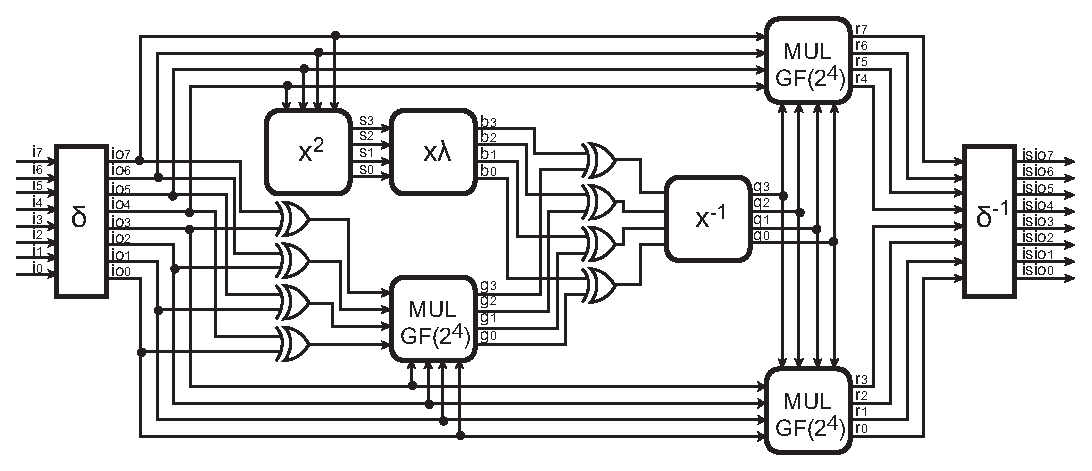
\includegraphics[width=3.4in]{eps/multiplicativeinversionmodule.eps}
   % \epsfxsize=3.4in
   % \epsffile{eps/multiplicativeinversionmodule.eps} 

  \caption{
  The illustration depicts the logic that is used to implement the multiplicative inversion in circuits and the aesbash.sh verification code.  
  }
  \label{fig:multiplicativeinversion}
  \end{center}
  \vskip -0.2in
\end{figure} 
The verification logic for the Multiplicative Inversion Module is reported in Table \ref{tab:aesmultiplicativeinversionmodule}, and this output was automatically generated by the script   {aestest\_multiplicativeinversion.sh}, which iterates through every input.  A single input can be evaluated by 
\begin{lstlisting}[language=bash]
#!/bin/sh
source aesbash.sh
aes_multiplicativeinversion "00000100"
\end{lstlisting}
where ``00000100" in the example above is the binary input representing 0x04.


\begin{table}[t]
 \caption{The pre-calculated multiplicative inversion module logic results }
  \label{tab:aesmultiplicativeinversionmodule}
\centering
%autogenerated by aestest_multiplicativeinversion via aestest_multiplicativeinversion.sh
\begin{tabular}{@{\hskip2pt}c@{\hskip2pt}@{\hskip2pt}c@{\hskip2pt}|@{\hskip2pt}c@{\hskip2pt}|@{\hskip2pt}c@{\hskip2pt}|@{\hskip2pt}c@{\hskip2pt}|@{\hskip2pt}c@{\hskip2pt}|@{\hskip2pt}c@{\hskip2pt}|@{\hskip2pt}c@{\hskip2pt}|@{\hskip2pt}c@{\hskip2pt}|@{\hskip2pt}c@{\hskip2pt}|@{\hskip2pt}c@{\hskip2pt}|@{\hskip2pt}c@{\hskip2pt}|@{\hskip2pt}c@{\hskip2pt}|@{\hskip2pt}c@{\hskip2pt}|@{\hskip2pt}c@{\hskip2pt}|@{\hskip2pt}c@{\hskip2pt}|@{\hskip2pt}c@{\hskip2pt}|}
 & 00 & 01 & 02 & 03 & 04 & 05 & 06 & 07 & 08 & 09 & 0a & 0b & 0c & 0d & 0e & 0f \\ 
 \hline
00 &00 & 01 & 8d & f6 & cb & 52 & 7b & d1 & e8 & 4f & 29 & c0 & b0 & e1 & e5 & c7 \\ 
 \hline
10 &74 & b4 & aa & 4b & 99 & 2b & 60 & 5f & 58 & 3f & fd & cc & ff & 40 & ee & b2 \\ 
 \hline
20 &3a & 6e & 5a & f1 & 55 & 4d & a8 & c9 & c1 & 0a & 98 & 15 & 30 & 44 & a2 & c2 \\ 
 \hline
30 &2c & 45 & 92 & 6c & f3 & 39 & 66 & 42 & f2 & 35 & 20 & 6f & 77 & bb & 59 & 19 \\ 
 \hline
40 &1d & fe & 37 & 67 & 2d & 31 & f5 & 69 & a7 & 64 & ab & 13 & 54 & 25 & e9 & 09 \\ 
 \hline
50 &ed & 5c & 05 & ca & 4c & 24 & 87 & bf & 18 & 3e & 22 & f0 & 51 & ec & 61 & 17 \\ 
 \hline
60 &16 & 5e & af & d3 & 49 & a6 & 36 & 43 & f4 & 47 & 91 & df & 33 & 93 & 21 & 3b \\ 
 \hline
70 &79 & b7 & 97 & 85 & 10 & b5 & ba & 3c & b6 & 70 & d0 & 06 & a1 & fa & 81 & 82 \\ 
 \hline
80 &83 & 7e & 7f & 80 & 96 & 73 & be & 56 & 9b & 9e & 95 & d9 & f7 & 02 & b9 & a4 \\ 
 \hline
90 &de & 6a & 32 & 6d & d8 & 8a & 84 & 72 & 2a & 14 & 9f & 88 & f9 & dc & 89 & 9a \\ 
 \hline
a0 &fb & 7c & 2e & c3 & 8f & b8 & 65 & 48 & 26 & c8 & 12 & 4a & ce & e7 & d2 & 62 \\ 
 \hline
b0 &0c & e0 & 1f & ef & 11 & 75 & 78 & 71 & a5 & 8e & 76 & 3d & bd & bc & 86 & 57 \\ 
 \hline
c0 &0b & 28 & 2f & a3 & da & d4 & e4 & 0f & a9 & 27 & 53 & 04 & 1b & fc & ac & e6 \\ 
 \hline
d0 &7a & 07 & ae & 63 & c5 & db & e2 & ea & 94 & 8b & c4 & d5 & 9d & f8 & 90 & 6b \\ 
 \hline
e0 &b1 & 0d & d6 & eb & c6 & 0e & cf & ad & 08 & 4e & d7 & e3 & 5d & 50 & 1e & b3 \\ 
 \hline
f0 &5b & 23 & 38 & 34 & 68 & 46 & 03 & 8c & dd & 9c & 7d & a0 & cd & 1a & 41 & 1c \\ 
 \hline
\end{tabular}
\end{table}




\subsection{Isomorphic Transform}
The isomorphic mapping exists to make the mathematics more efficient in the circuit sense.  AES involves arithmetic on \(GF(2^8)\) elements, and from the hardware perspective, the naive approach is to use lookup tables.  The mapping of the operations into a composite field via an isomorphic transform allows for a decreased complexity in circuit logic at the cost of the isomorphic transform circuits. 



\subsubsection{Isomorphic Mapping Module}

In Figure \ref{fig:multiplicativeinversion}, the inputs to the isomorphic unit are labeled as \(i_x\), where \(_x\) is the bit line number.  The outputs of the isomorphic unit are labelled as \(io\).

\begin{equation}
\label{matrix:isomorph}
\delta \times i =
 \begin{pmatrix}
  1 & 0 & 1 & 0 & 0 & 0 & 0 & 0 \\
  1 & 1 & 0 & 1 & 1 & 1 & 1 & 0 \\
  1 & 0 & 1 & 0 & 1 & 1 & 0 & 0 \\
  1 & 0 & 1 & 0 & 1 & 1 & 1 & 0 \\
  1 & 1 & 0 & 0 & 0 & 1 & 1 & 0 \\
  1 & 0 & 0 & 1 & 1 & 1 & 1 & 0 \\
  0 & 1 & 0 & 1 & 0 & 0 & 1 & 0 \\
  0 & 1 & 0 & 0 & 0 & 0 & 1 & 1
 \end{pmatrix}
 \times
 \begin{pmatrix}
  i_7 \\
  i_6 \\
  i_5 \\
  i_4 \\
  i_3 \\
  i_2 \\
  i_1 \\
  i_0 
 \end{pmatrix}
\end{equation}
In equation (\ref{matrix:isomorph}), the input bit \(i_x\) is mapped to the isomorphic field described by \(\delta\), thus, \(io=\delta \times i\).  This results in
\begin{equation}
\label{matrix:isomorphimpl}
\delta \times i =
 \begin{pmatrix}
  io_7 \\
  io_6 \\
  io_5 \\
  io_4 \\
  io_3 \\
  io_2 \\
  io_1 \\
  io_0 
 \end{pmatrix}
  = 
  \begin{pmatrix}
  \multicolumn{8}{c}{i_7 \oplus i_5} \\
  \multicolumn{8}{c}{i_7 \oplus i_6 \oplus i_4 \oplus i_3 \oplus i_2 } \\
  \multicolumn{8}{c}{i_7 \oplus i_5 \oplus i_3 \oplus i_2 } \\
  \multicolumn{8}{c}{i_7 \oplus i_5 \oplus i_3 \oplus i_2 \oplus i_1 } \\
  \multicolumn{8}{c}{i_7 \oplus i_6 \oplus i_2 \oplus i_1 } \\
  \multicolumn{8}{c}{i_7 \oplus i_4 \oplus i_3 \oplus i_2 \oplus i_1} \\
  \multicolumn{8}{c}{i_6 \oplus i_4 \oplus i_1} \\
  \multicolumn{8}{c}{i_6 \oplus i_1 \oplus i_0} \\
 \end{pmatrix},
\end{equation}
where each ``1" in the isomorphic field \(\delta\) corresponds to an XOR, which results in the logic shown in equation (\ref{matrix:isomorphimpl}).
\begin{table}[t]
 \caption{The pre-calculated isomorphic mapping module logic verification }
  \label{tab:aesisomorphicmodule}
\centering
\begin{tabular}{@{\hskip3pt}c@{\hskip3pt}|@{\hskip3pt}c@{\hskip3pt}|@{\hskip3pt}c@{\hskip3pt}|@{\hskip3pt}c@{\hskip3pt}|@{\hskip3pt}c@{\hskip3pt}|@{\hskip3pt}c@{\hskip3pt}|@{\hskip3pt}c@{\hskip3pt}|@{\hskip3pt}c@{\hskip3pt}|@{\hskip3pt}c@{\hskip3pt}|@{\hskip3pt}c@{\hskip3pt}|@{\hskip3pt}c@{\hskip3pt}|@{\hskip3pt}c@{\hskip3pt}|@{\hskip3pt}c@{\hskip3pt}|@{\hskip3pt}c@{\hskip3pt}|@{\hskip3pt}c@{\hskip3pt}|@{\hskip3pt}c@{\hskip3pt}|@{\hskip3pt}c@{\hskip3pt}|}
 & 00 & 01 & 02 & 03 & 04 & 05 & 06 & 07 & 08 & 09 & 0a & 0b & 0c & 0d & 0e & 0f \\ 
 \hline
00 &00 & 01 & 5f & 5e & 7c & 7d & 23 & 22 & 74 & 75 & 2b & 2a & 08 & 09 & 57 & 56 \\ 
 \hline
10 &46 & 47 & 19 & 18 & 3a & 3b & 65 & 64 & 32 & 33 & 6d & 6c & 4e & 4f & 11 & 10 \\ 
 \hline
20 &b0 & b1 & ef & ee & cc & cd & 93 & 92 & c4 & c5 & 9b & 9a & b8 & b9 & e7 & e6 \\ 
 \hline
30 &f6 & f7 & a9 & a8 & 8a & 8b & d5 & d4 & 82 & 83 & dd & dc & fe & ff & a1 & a0 \\ 
 \hline
40 &4b & 4a & 14 & 15 & 37 & 36 & 68 & 69 & 3f & 3e & 60 & 61 & 43 & 42 & 1c & 1d \\ 
 \hline
50 &0d & 0c & 52 & 53 & 71 & 70 & 2e & 2f & 79 & 78 & 26 & 27 & 05 & 04 & 5a & 5b \\ 
 \hline
60 &fb & fa & a4 & a5 & 87 & 86 & d8 & d9 & 8f & 8e & d0 & d1 & f3 & f2 & ac & ad \\ 
 \hline
70 &bd & bc & e2 & e3 & c1 & c0 & 9e & 9f & c9 & c8 & 96 & 97 & b5 & b4 & ea & eb \\ 
 \hline
80 &fc & fd & a3 & a2 & 80 & 81 & df & de & 88 & 89 & d7 & d6 & f4 & f5 & ab & aa \\ 
 \hline
90 &ba & bb & e5 & e4 & c6 & c7 & 99 & 98 & ce & cf & 91 & 90 & b2 & b3 & ed & ec \\ 
 \hline
a0 &4c & 4d & 13 & 12 & 30 & 31 & 6f & 6e & 38 & 39 & 67 & 66 & 44 & 45 & 1b & 1a \\ 
 \hline
b0 &0a & 0b & 55 & 54 & 76 & 77 & 29 & 28 & 7e & 7f & 21 & 20 & 02 & 03 & 5d & 5c \\ 
 \hline
c0 &b7 & b6 & e8 & e9 & cb & ca & 94 & 95 & c3 & c2 & 9c & 9d & bf & be & e0 & e1 \\ 
 \hline
d0 &f1 & f0 & ae & af & 8d & 8c & d2 & d3 & 85 & 84 & da & db & f9 & f8 & a6 & a7 \\ 
 \hline
e0 &07 & 06 & 58 & 59 & 7b & 7a & 24 & 25 & 73 & 72 & 2c & 2d & 0f & 0e & 50 & 51 \\ 
 \hline
f0 &41 & 40 & 1e & 1f & 3d & 3c & 62 & 63 & 35 & 34 & 6a & 6b & 49 & 48 & 16 & 17 \\ 
 \hline
\end{tabular}
\end{table}
The verification logic for the Isomorphic Mapping Module is reported in Table \ref{tab:aesisomorphicmodule}, and this output was automatically generated by the script   {aestest\_isomorphic.sh}, which iterates through every input.  A single input can be evaluated by 
\begin{lstlisting}[language=bash]
#!/bin/sh
source aesbash.sh
aes_isomorphic "00000100"
\end{lstlisting}
where ``00000100" in the example above is the binary input representing 0x04.

\subsubsection{Inverse Isomorphic Module}
In Figure \ref{fig:multiplicativeinversion}, the inputs to the isomorphic inversion unit are labeled as \(r_x\), where \(_x\) is the bit line number.  The outputs of the isomorphic unit are labelled as \(isio\).
\begin{equation}
\label{matrix:invisomorph}
\delta^{-1} \times r
=
 \begin{pmatrix}
  1 & 1 & 1 & 0 & 0 & 0 & 1 & 0 \\
  0 & 1 & 0 & 0 & 0 & 1 & 0 & 0 \\
  0 & 1 & 1 & 0 & 0 & 0 & 1 & 0 \\
  0 & 1 & 1 & 1 & 0 & 1 & 1 & 0 \\
  0 & 0 & 1 & 1 & 1 & 1 & 1 & 0 \\
  1 & 0 & 0 & 1 & 1 & 1 & 1 & 0 \\
  0 & 0 & 1 & 1 & 0 & 0 & 0 & 0 \\
  0 & 1 & 1 & 1 & 0 & 1 & 0 & 1
 \end{pmatrix}
 \times
 \begin{pmatrix}
  r_7 \\
  r_6 \\
  r_5 \\
  r_4 \\
  r_3 \\
  r_2 \\
  r_1 \\
  r_0 
 \end{pmatrix}
\end{equation}
In equation (\ref{matrix:invisomorph}), the input bit \(r_x\) is mapped to the isomorphic inversion field described by \(\delta^{-1}\), thus, \(io=\delta^{-1} \times i\).  This results in
\begin{equation}
\label{matrix:invisomorphimpl}
\delta^{-1} \times r
 = 
 \begin{pmatrix}
  isio_7 \\
  isio_6 \\
  isio_5 \\
  isio_4 \\
  isio_3 \\
  isio_2 \\
  isio_1 \\
  isio_0 
 \end{pmatrix}
 = 
  \begin{pmatrix}
  \multicolumn{8}{c}{r_7 \oplus r_6 \oplus r_5 \oplus r_1} \\
  \multicolumn{8}{c}{r_6 \oplus r_2  } \\
  \multicolumn{8}{c}{r_6 \oplus r_5 \oplus r_1 } \\
  \multicolumn{8}{c}{r_6 \oplus r_5 \oplus r_4 \oplus r_2 \oplus r_1 } \\
  \multicolumn{8}{c}{r_5 \oplus r_4 \oplus r_3 \oplus r_2 \oplus r_1 } \\
  \multicolumn{8}{c}{r_7 \oplus r_4 \oplus r_3 \oplus r_2 \oplus r_1} \\
  \multicolumn{8}{c}{r_5 \oplus r_4 } \\
  \multicolumn{8}{c}{r_6 \oplus r_5 \oplus r_4 \oplus r_2 \oplus r_0} \\
 \end{pmatrix}
\end{equation}
where each ``1" in the isomorphic field \(\delta^{-1}\) corresponds to an XOR, which results in the logic shown in equation (\ref{matrix:invisomorphimpl}).

\begin{table}[t]
 \caption{The pre-calculated inverse isomorphic mapping module logic verification }
  \label{tab:invaesisomorphicmodule}
\centering
%autogenerated by aestest_isomorphicinv via aestest_isomorphicinv.sh
\begin{tabular}{@{\hskip3pt}c@{\hskip3pt}|@{\hskip3pt}c@{\hskip3pt}|@{\hskip3pt}c@{\hskip3pt}|@{\hskip3pt}c@{\hskip3pt}|@{\hskip3pt}c@{\hskip3pt}|@{\hskip3pt}c@{\hskip3pt}|@{\hskip3pt}c@{\hskip3pt}|@{\hskip3pt}c@{\hskip3pt}|@{\hskip3pt}c@{\hskip3pt}|@{\hskip3pt}c@{\hskip3pt}|@{\hskip3pt}c@{\hskip3pt}|@{\hskip3pt}c@{\hskip3pt}|@{\hskip3pt}c@{\hskip3pt}|@{\hskip3pt}c@{\hskip3pt}|@{\hskip3pt}c@{\hskip3pt}|@{\hskip3pt}c@{\hskip3pt}|@{\hskip3pt}c@{\hskip3pt}|}
 & 00 & 01 & 02 & 03 & 04 & 05 & 06 & 07 & 08 & 09 & 0a & 0b & 0c & 0d & 0e & 0f \\ 
 \hline
00 &00 & 01 & bc & bd & 5d & 5c & e1 & e0 & 0c & 0d & b0 & b1 & 51 & 50 & ed & ec \\ 
 \hline
10 &1f & 1e & a3 & a2 & 42 & 43 & fe & ff & 13 & 12 & af & ae & 4e & 4f & f2 & f3 \\ 
 \hline
20 &bb & ba & 07 & 06 & e6 & e7 & 5a & 5b & b7 & b6 & 0b & 0a & ea & eb & 56 & 57 \\ 
 \hline
30 &a4 & a5 & 18 & 19 & f9 & f8 & 45 & 44 & a8 & a9 & 14 & 15 & f5 & f4 & 49 & 48 \\ 
 \hline
40 &f1 & f0 & 4d & 4c & ac & ad & 10 & 11 & fd & fc & 41 & 40 & a0 & a1 & 1c & 1d \\ 
 \hline
50 &ee & ef & 52 & 53 & b3 & b2 & 0f & 0e & e2 & e3 & 5e & 5f & bf & be & 03 & 02 \\ 
 \hline
60 &4a & 4b & f6 & f7 & 17 & 16 & ab & aa & 46 & 47 & fa & fb & 1b & 1a & a7 & a6 \\ 
 \hline
70 &55 & 54 & e9 & e8 & 08 & 09 & b4 & b5 & 59 & 58 & e5 & e4 & 04 & 05 & b8 & b9 \\ 
 \hline
80 &84 & 85 & 38 & 39 & d9 & d8 & 65 & 64 & 88 & 89 & 34 & 35 & d5 & d4 & 69 & 68 \\ 
 \hline
90 &9b & 9a & 27 & 26 & c6 & c7 & 7a & 7b & 97 & 96 & 2b & 2a & ca & cb & 76 & 77 \\ 
 \hline
a0 &3f & 3e & 83 & 82 & 62 & 63 & de & df & 33 & 32 & 8f & 8e & 6e & 6f & d2 & d3 \\ 
 \hline
b0 &20 & 21 & 9c & 9d & 7d & 7c & c1 & c0 & 2c & 2d & 90 & 91 & 71 & 70 & cd & cc \\ 
 \hline
c0 &75 & 74 & c9 & c8 & 28 & 29 & 94 & 95 & 79 & 78 & c5 & c4 & 24 & 25 & 98 & 99 \\ 
 \hline
d0 &6a & 6b & d6 & d7 & 37 & 36 & 8b & 8a & 66 & 67 & da & db & 3b & 3a & 87 & 86 \\ 
 \hline
e0 &ce & cf & 72 & 73 & 93 & 92 & 2f & 2e & c2 & c3 & 7e & 7f & 9f & 9e & 23 & 22 \\ 
 \hline
f0 &d1 & d0 & 6d & 6c & 8c & 8d & 30 & 31 & dd & dc & 61 & 60 & 80 & 81 & 3c & 3d \\ 
 \hline
\end{tabular}
\end{table}
The verification logic for the Inverse Isomorphic Mapping Module is reported in Table \ref{tab:invaesisomorphicmodule}, and this output was automatically generated by the script   {aestest\_invisomorphic.sh}, which iterates through every input.  A single input can be evaluated by 
\begin{lstlisting}[language=bash]
#!/bin/sh
source aesbash.sh
aes_isomorphicinv "00000100"
\end{lstlisting}
where ``00000100" in the example above is the binary input representing 0x04.


\subsection{\(GF(2^4)\) Addition}
Addition in a Galois Field, \(GF(2)\), is simply the XOR between elements.  

\subsection{\(GF(2^2)\) Multiplication}
\label{subsec:gf22mul}
The \(GF(2^2)\) Multiplication Module operates on two, 2-bit inputs and results in a 2-bit output. For the elements in \(GF(2^2)\), let the output, k, be the product of inputs a and b, so that \(k=ab\), where \(k=\{k_1,k_0\}\), \(a=\{a_1,a_0\}\) and \(b=\{b_1,b_0\}\).  Mapping the inputs into a \(GF(2)\) polynomial results in
\begin{align}
k&=k_1x+k_0=\left(a_1a_0\right)\left(b_1b_0\right)\nonumber\\
k&=k_1x+k_0=\left(a_1x +a_0\right)\left(b_1x+b_0\right)\\
k&=k_1x+k_0=\left(a_1b_1x^2+a_1b_0x+a_0b_1x+a_0b_0\right) \nonumber
\end{align}
which can be further reduced because \(x^2=x+1\).  The resulting equation is 
\begin{align}
\label{equ:GFF22mul:mathfinal}
k&=k_1x+k_0=a_1b_1\left(x+1\right)+a_1b_0x+a_0b_1x+a_0b_0 \nonumber\\
&=\left(a_1b_1+a_1b_0+a_0b_1\right)x+\left(a_1b_1+a_0b_0\right),
\end{align}
which can be implemented as AND and XOR logic.  The logical representation of (\ref{equ:GFF22mul:mathfinal}) is 
{\renewcommand{\arraystretch}{1.0}%
\begin{align}
\label{equ:GFF22mul:logicfinal}
%\resizebox{\columnwidth}{!}{
\scalebox{1}{
\( k = \left\{
\begin{array}{l}
         k_1=a_1b_1\oplus a_1b_0 \oplus a_0b_1\\
         k_0=a_1b_1 \oplus a_0b_0\\
\end{array}\right.
\)
}
\end{align} 
}
and this logic is implemented in Figure \ref{fig:gf22mul}.  
\begin{figure}[t]
  \begin{center}
  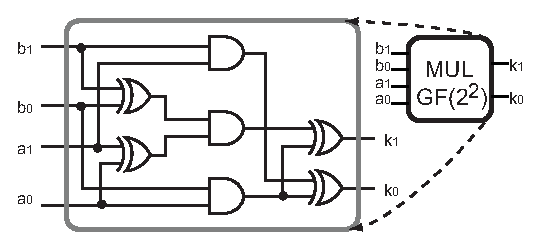
\includegraphics[width=3.2in]{eps/gf22mul.eps}
  %  \epsfxsize=3.2in
  %  \epsffile{eps/gf22mul.eps} 

  \caption{
  The illustration reports the implementation logic structure of the \(GF(2^2)\) multiplication module.  
  }
  \label{fig:gf22mul}
  \end{center}
  \vskip -0.2in
\end{figure} 
%%%%%%%%%%%%%%%%%%%%%%%%%%
\begin{table}[t]
 \caption{The pre-calculated \(GF(2^2)\) Multiplication Module logic verification }
  \label{tab:gf22mul}
\centering
\begin{tabular}{c|c|c|c|c|}
 & 0 & 1 & 2 & 3 \\ 
 \hline
0 &0 & 0 & 0 & 0 \\ 
 \hline
1 &0 & 1 & 2 & 3 \\ 
 \hline
2 &0 & 2 & 3 & 1 \\ 
 \hline
3 &0 & 3 & 1 & 2 \\ 
 \hline
\end{tabular}
\end{table}

The verification of the logic for the \(GF(2^2)\) Multiplication Module is reported in Table \ref{tab:gf22mul}, and this output was automatically generated by the script {aestest\_multGF22.sh}, which iterates through every input. The function expects as single 4-bit input which represents the two, 2-bit values being multiplied, as \(a_1a_0b_1b_0\).  This is due to a limitation in the bashbignumbers.sh dependency which has nibble boundaries.  A single input can be evaluated by 
\begin{lstlisting}[language=bash]
#!/bin/sh
source aesbash.sh
aes_multGF2 "0111"
\end{lstlisting}
where ``0111" in the example above is the binary input of \(a=\{0,1\}\) and \(b=\{1,1\}\) resulting in an output of \(k=\{1,1\}\).

\subsection{\(GF(2^2)\) Multiplication by constant}
\label{subsec:gf22constantmul}
The multiplication by a constant, \(\varphi\), is a special case of the \(GF(2^2)\) Multiplication Module described in Section \ref{subsec:gf22mul}.  The constant \(\varphi=\{1,0\}\) is a fixed value on the ``b" input to \(GF(2^2)\) multiplication.  Starting from equation (\ref{equ:GFF22mul:mathfinal}), we can reduce the logic to
\begin{align}
\label{equ:GFF22mulconstant:mathfinal}
k&=\left(a_1+a_0\right)x+a_1,
\end{align}
which reduces to logic based on an XOR as
{\renewcommand{\arraystretch}{1.0}%
\begin{align}
\label{equ:GFF22mulconst:logicfinal}
%\resizebox{\columnwidth}{!}{
\scalebox{1}{
\( k = \left\{
\begin{array}{l}
         k_1=a_1\oplus a_0\\
         k_0=a_1\\
\end{array}\right.,
\)
}
\end{align} 
}
and test vector was not created for this module as it can be done by inspection.

\subsection{\(GF(2^4)\) Multiplication}
\label{subsec:mulGF24}
The \(GF(2^4)\) Multiplication Module operates on two, 4-bit inputs and results in a 4-bit output. For the elements in \(GF(2^4)\), let the output, k, be the product of inputs a and b, so that \(k=ab\), where \(k=\{k_3,k_2,k_1,k_0\}\), \(a=\{a_3,a_2,a_1,a_0\}\) and \(b=\{b_3,b_2,b_1,b_0\}\). Mapping the inputs into a \(GF(2)\) polynomial results in

\begin{align}
\label{equ:GFF24mul}
k&=\underbrace{k_3k_2}_{k_H}\underbrace{k_1k_0}_{k_L}=\big(\underbrace{a_3a_2}_{\mathclap{a_H}} \underbrace{a_1a_0}_{\mathclap{a_L}}\big)\big(\underbrace{b_3b_2}_{\mathclap{b_H}} \underbrace{b_1b_0}_{\mathclap{b_L}}\big)\nonumber\\
&={k_H}x+{k_L}=\left(a_Hx+a_L\right)\left(b_Hx+b_L\right)\\
&=\left(a_Hb_H\right)x^2+\left(a_Hb_L+a_Lb_H\right)x + a_Lb_L \nonumber
\end{align}
to which \(x^2=x+\varphi\) can be substituted.  The \(\varphi\) constant is defined in Section \ref{subsec:gf22constantmul}.  The resulting equation is 
\begin{align}
\label{equ:GFF24mullogic}
k&=\left(a_Hb_H\right)\left(x+\varphi\right)+\left(a_Hb_L+a_Lb_H\right)x+a_Lb_L \nonumber \\
&=\left(a_Hb_H +a_Hb_L+a_Lb_H \right)x+a_Hb_H\varphi+a_Lb_L
\end{align}
and this logic is implemented in the circuit illustrated in Figure \ref{fig:gf24mul}.  The verification logic for the \(GF(2^4)\) Multiplication Module is reported in Table \ref{tab:mulGF24module}, and this output was automatically generated by the script {aestest\_multGF24.sh}, which iterates through every input.  A single input can be evaluated by 
\begin{lstlisting}[language=bash]
#!/bin/sh
source aesbash.sh
aes_multGF24 "00100100"
\end{lstlisting}
where ``00100100" in the example above is the binary input of \(a=\{0,0,1,0\}\) and \(b=\{0,1,0,0\}\) resulting in an output of \(k=\{1,0,0,0\}\).

\begin{table}[t]
 \caption{The pre-calculated \(GF(2^4)\) Multiplication Module logic verification }
  \label{tab:mulGF24module}
\centering
%autogenerated by aestest_multGF24 via aestest_multGF24.sh
\begin{tabular}{@{\hskip3pt}c@{\hskip3pt}|@{\hskip3pt}c@{\hskip3pt}|@{\hskip3pt}c@{\hskip3pt}|@{\hskip3pt}c@{\hskip3pt}|@{\hskip3pt}c@{\hskip3pt}|@{\hskip3pt}c@{\hskip3pt}|@{\hskip3pt}c@{\hskip3pt}|@{\hskip3pt}c@{\hskip3pt}|@{\hskip3pt}c@{\hskip3pt}|@{\hskip3pt}c@{\hskip3pt}|@{\hskip3pt}c@{\hskip3pt}|@{\hskip3pt}c@{\hskip3pt}|@{\hskip3pt}c@{\hskip3pt}|@{\hskip3pt}c@{\hskip3pt}|@{\hskip3pt}c@{\hskip3pt}|@{\hskip3pt}c@{\hskip3pt}|@{\hskip3pt}c@{\hskip3pt}|}
 & 0 & 1 & 2 & 3 & 4 & 5 & 6 & 7 & 8 & 9 & a & b & c & d & e & f \\ 
 \hline
0 &0 & 0 & 0 & 0 & 0 & 0 & 0 & 0 & 0 & 0 & 0 & 0 & 0 & 0 & 0 & 0 \\ 
 \hline
1 &0 & 1 & 2 & 3 & 4 & 5 & 6 & 7 & 8 & 9 & a & b & c & d & e & f \\ 
 \hline
2 &0 & 2 & 3 & 1 & 8 & a & b & 9 & c & e & f & d & 4 & 6 & 7 & 5 \\ 
 \hline
3 &0 & 3 & 1 & 2 & c & f & d & e & 4 & 7 & 5 & 6 & 8 & b & 9 & a \\ 
 \hline
4 &0 & 4 & 8 & c & 6 & 2 & e & a & b & f & 3 & 7 & d & 9 & 5 & 1 \\ 
 \hline
5 &0 & 5 & a & f & 2 & 7 & 8 & d & 3 & 6 & 9 & c & 1 & 4 & b & e \\ 
 \hline
6 &0 & 6 & b & d & e & 8 & 5 & 3 & 7 & 1 & c & a & 9 & f & 2 & 4 \\ 
 \hline
7 &0 & 7 & 9 & e & a & d & 3 & 4 & f & 8 & 6 & 1 & 5 & 2 & c & b \\ 
 \hline
8 &0 & 8 & c & 4 & b & 3 & 7 & f & d & 5 & 1 & 9 & 6 & e & a & 2 \\ 
 \hline
9 &0 & 9 & e & 7 & f & 6 & 1 & 8 & 5 & c & b & 2 & a & 3 & 4 & d \\ 
 \hline
a &0 & a & f & 5 & 3 & 9 & c & 6 & 1 & b & e & 4 & 2 & 8 & d & 7 \\ 
 \hline
b &0 & b & d & 6 & 7 & c & a & 1 & 9 & 2 & 4 & f & e & 5 & 3 & 8 \\ 
 \hline
c &0 & c & 4 & 8 & d & 1 & 9 & 5 & 6 & a & 2 & e & b & 7 & f & 3 \\ 
 \hline
d &0 & d & 6 & b & 9 & 4 & f & 2 & e & 3 & 8 & 5 & 7 & a & 1 & c \\ 
 \hline
e &0 & e & 7 & 9 & 5 & b & 2 & c & a & 4 & d & 3 & f & 1 & 8 & 6 \\ 
 \hline
f &0 & f & 5 & a & 1 & e & 4 & b & 2 & d & 7 & 8 & 3 & c & 6 & 9 \\ 
 \hline
\end{tabular}
\end{table}

\begin{figure}[t]
  \begin{center}
  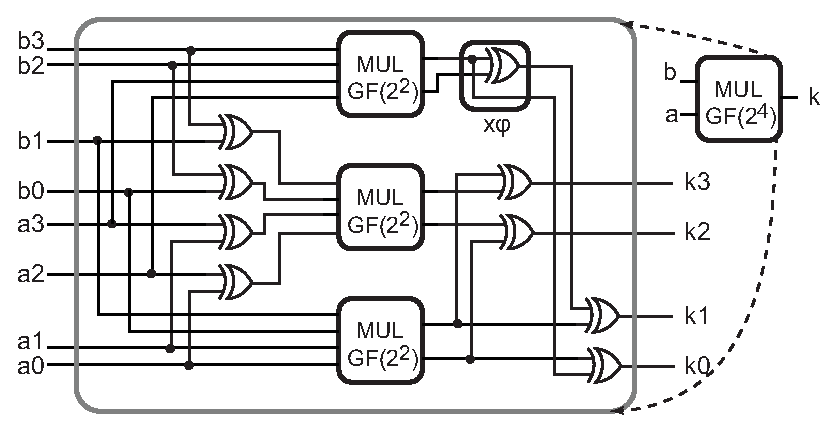
\includegraphics[width=3.2in]{eps/gf24mul.eps}
   % \epsfxsize=3.2in
   % \epsffile{eps/gf24mul.eps} 

  \caption{
  The illustration reports the implementation logic structure of the \(GF(2^4)\) multiplication module.  Note the additional XOR on the most significant multiplier that creates the constant multiplication, \(x\varphi\), in \(GF(2^2)\) that is described in Section \ref{subsec:gf22constantmul}.   
  }
  \label{fig:gf24mul}
  \end{center}
  \vskip -0.2in
\end{figure} 


\subsection{\(GF(2^4)\) Squaring Module}
\label{subsec:sqrGF24}
The \(GF(2^4)\) Squaring Module operates one 4-bit input and results in a 4-bit output. For the elements in \(GF(2^4)\), let the output, k, be the product of input \(a^2\), so that \(k=aa\), where \(k=\{k_3,k_2,k_1,k_0\}\), and \(a=\{a_3,a_2,a_1,a_0\}\). Mapping the inputs into a \(GF(2)\) polynomial results in

\begin{align}
\label{equ:sqrGF24}
k&=\underbrace{k_3k_2}_{k_H}\underbrace{k_1k_0}_{k_L}=\big(\underbrace{a_3a_2}_{\mathclap{a_H}} \underbrace{a_1a_0}_{\mathclap{a_L}}\big)^2\nonumber\\
&={k_H}x+{k_L}=\left(a_Hx+a_L\right)^2\nonumber \\
&=\left(a_Hb_H\right)x^2+\left(a_Hb_L+a_Lb_H\right)x + a_Lb_L \\
&={a_H}^2x^2+{a_L}^2.\nonumber
\end{align}
The naive approach would be to simply put the same values into the \(a\) and \(b\) inputs of the \(GF(2^4)\) Multiplication Module described in Section \ref{subsec:mulGF24}; however, the circuit complexity can be decreased using the reductions described in equation (\ref{eqn:GFdecomposition}).  The \(x^2\) term can be reduced by setting \(x^2=x+\varphi\), resulting in
\begin{align}
\label{equ:sqrGF24logic}
k&={a_H}^2x^2+{a_L}^2\nonumber\\
&={a_H}^2\left(x+\varphi \right)+{a_L}^2\nonumber\\
&=\underbrace{{a_H}^2x}_{k_H}+\underbrace{{a_H}^2 \varphi +{a_L}^2}_{k_L}
\end{align}
which is now in terms of \(GF(2^2)\).  Starting from the high term, \(k_H\), and using the substitutions in (\ref{eqn:GFdecomposition}) we can show that
\begin{align}
\label{equ:sqrGF22kh}
k_H&=a_H^2=(a_3a_2)^2\nonumber \\
k_H&=a_H^2=(a_3x+a_2)^2\nonumber\\
k_H&=a_3^2x^2+a_3a_2x+a_3a_2x+a_2^2=a_3x^2+a_2\\
k_H&=a_3(x+1)+a_2\nonumber \\
k_H&=k_3x+k_2=\underbrace{a_3x}_{k_3}+\underbrace{a_3+a_2}_{k_2}. \nonumber
\end{align}
Continuing the decomposition with the low term, \(k_L\), where \(\varphi=\{10\}\), results in 
\begin{align}
\label{equ:sqrGF22kl}
k_L&=a_H^2\varphi+a_L^2=(a_3a_2)^2\{10\}+(a_1a_0)^2 \nonumber \\
k_L&=\left(a_3x+a_2\right)^2\left(\{1\}x+\{0\}\right)+\left(a_1x+a_0\right)^2 \nonumber \\
k_L&=\left(a_3^2x^2+a_3a_2x+a_2a_3x+a_2^2\right)x \nonumber \\
   &+\left(a_1^2x^2+a_1a_0x+a_0a_1x+a_0^2\right)\\
k_L&=a_3x^3+a_2x+a_1x^2+a_0\nonumber \\
k_L&=a_3(1)+a_2x+a_1(x+1)+a_0 \nonumber \\
k_L&=k_1x+k_0=(a_2+a_1)x+(a_3+a_1+a_0),\nonumber
\end{align}
where the simplification is from \(x^3=x^2+x=(x+1)+x=1\).  Combining (\ref{equ:sqrGF22kh}) and (\ref{equ:sqrGF22kl}) results in the final logic equation of

{\renewcommand{\arraystretch}{1.0}%
\begin{align}
\label{equ:sqrGF24:logicfinal}
%\resizebox{\columnwidth}{!}{
\scalebox{1}{
\( k = \left\{
\begin{array}{l}
         k_3=a_3\\
         k_2=a_3 \oplus a_2\\
         k_1=a_2\oplus a_1\\
         k_0=a_3 \oplus a_1 \oplus a_0\\
\end{array}\right.
\)
}
\end{align} 
}
which can be implemented as 4 XOR gates. The logic is implemented in the circuit illustrated in Figure \ref{fig:gf24sqr}.  The verification logic for the \(GF(2^4)\) Squaring Module is reported in Table \ref{tab:sqrGF24}, and this output was automatically generated by the script {aestest\_sqrGF24.sh}, which iterates through every input.  A single input can be evaluated by 
\begin{lstlisting}[language=bash]
#!/bin/sh
source aesbash.sh
aes_squarerGF24 "0100"
\end{lstlisting}
where ``0100" in the example above is the binary input of \(a=\{0,1,0,0\}\) resulting in an output of \(k=\{0,1,1,0\}\).

\begin{figure}[t]
  \begin{center}
  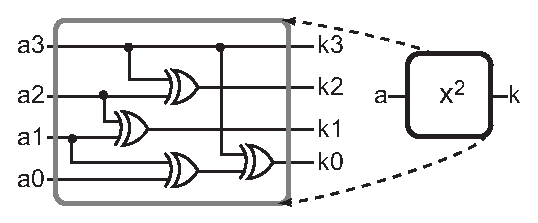
\includegraphics[width=3.2in]{eps/gf24sqr.eps}
   % \epsfxsize=3.2in
    %\epsffile{eps/gf24sqr.eps} 

  \caption{
  The illustration reports the implementation logic structure of the \(GF(2^4)\) squaring module.     
  }
  \label{fig:gf24sqr}
  \end{center}
  \vskip -0.2in
\end{figure} 


\begin{table}[t]
 \caption{The pre-calculated \(GF(2^4)\) Squarer logic verification}
  \label{tab:sqrGF24}
\centering

%autogenerated by aestest_squarerGF24 via aestest_sqrGF24.sh
\begin{tabular}{@{\hskip3pt}c@{\hskip3pt}|@{\hskip3pt}c@{\hskip3pt}|@{\hskip3pt}c@{\hskip3pt}|@{\hskip3pt}c@{\hskip3pt}|@{\hskip3pt}c@{\hskip3pt}|@{\hskip3pt}c@{\hskip3pt}|@{\hskip3pt}c@{\hskip3pt}|@{\hskip3pt}c@{\hskip3pt}|@{\hskip3pt}c@{\hskip3pt}|@{\hskip3pt}c@{\hskip3pt}|@{\hskip3pt}c@{\hskip3pt}|@{\hskip3pt}c@{\hskip3pt}|@{\hskip3pt}c@{\hskip3pt}|@{\hskip3pt}c@{\hskip3pt}|@{\hskip3pt}c@{\hskip3pt}|@{\hskip3pt}c@{\hskip3pt}|@{\hskip3pt}c@{\hskip3pt}|}
 \hline
input & 0 & 1 & 2 & 3 & 4 & 5 & 6 & 7 & 8 & 9 & a & b & c & d & e & f \\ 
 \hline
output & 0 & 1 & 3 & 2 & 6 & 7 & 5 & 4 & d & c & e & f & b & a & 8 & 9 \\ 
 \hline
\end{tabular}
\end{table}


\subsection{\(GF(2^4)\) Multiplication by constant}
The \(GF(2^4)\) Multiplication by Constant Module operates one 4-bit input, a 4-bit constant and results in a 4-bit output. For the elements in \(GF(2^4)\), let the output, k, be the product of input \(a^2\), so that \(k=a\lambda\), where \(k=\{k_3,k_2,k_1,k_0\}\), \(a=\{a_3,a_2,a_1,a_0\}\) and \(\lambda=\{1100\}\). Mapping the inputs into a \(GF(2)\) polynomial results in

\begin{align}
\label{equ:mulconGF24}
k&=\underbrace{k_3k_2}_{k_H}\underbrace{k_1k_0}_{k_L}={k_H}x+{k_L}\nonumber\\
&={k_H}x+{k_L}=\big(\underbrace{a_3a_2}_{\mathclap{a_H}} \underbrace{a_1a_0}_{\mathclap{a_L}}\big)\big\{\underbrace{11}_{\mathclap{\lambda_H}} \underbrace{00}_{\mathclap{\lambda_L}}\big\}\nonumber\\
&=\left({a_H}x+{a_L}\right)\left({\lambda_H}x+{\lambda_L}\right)\nonumber\\
&={a_H}{\lambda_H}x^2+{a_L}{\lambda_H}x,
\end{align}
where \({\lambda_L}=\{00\}\), which cancels out many of the terms.  As with the squaring circuit, the naive approach would be to simply put the same values into the \(a\) and \(b\) inputs of the \(GF(2^4)\) Multiplication Module described in Section \ref{subsec:mulGF24}; however, the circuit complexity can be decreased using the reductions described in equation (\ref{eqn:GFdecomposition}). The substitution of \(x^2=x+\varphi\) reduces equation (\ref{equ:mulconGF24}) to
\begin{align}
\label{equ:mulconGF24reduce}
k&={a_H}{\lambda_H}\left(x+\varphi\right)+{a_L}{\lambda_H}x\nonumber\\
k&=\big(\underbrace{a_H\lambda_H+a_L\lambda_H}_{\mathclap{k_H}}\big)x+\big(\underbrace{a_H\lambda_H \varphi}_{\mathclap{k_L}}\big),
\end{align}
where \(k_H\) and \(k_L\) can be further reduced.  Starting with the \(k_H\) term in \ref{equ:mulconGF24reduce}, the reduction follow as

\begin{align}
\label{equ:mulconGF24reducekh}
k_H=&k_3x+k_2 \nonumber \\
=&a_H \lambda_H+a_L\lambda_H\nonumber\\
=&\left(a_3a_2\right)\left\{11\right\}+\left(a_1a_0\right)\left\{11\right\}\nonumber\\
=&\left(a_3x+a_2\right)\left(x+1\right)+\left(a_1x+a_0\right)\left(x+1\right)\nonumber\\
=&\left(a_3\right)x^2+\left(a_3+a_2\right)x+a_2\nonumber\\
&+a_1x^2+\left(a_1+a_0\right)x+a_0 : x^2=x+1\\
=&a_3\left(x+1\right)+\left(a_3+a_2\right)x+a_2\nonumber\\
&+a_1\left(x+1\right)+\left(a_1+a_0\right)x+a_0\nonumber\\
=&\left(a_3+a_3+a_2+a_1+a_1+a_0\right)x\nonumber\\
&+\left(a_3+a_2+a_1+a_0\right)\nonumber\\
=&k_3x+k_2=\left(a_2+a_0\right)x+\left(a_3+a_2+a_1+a_0\right).\nonumber
\end{align}
The \(k_L\) term can be decomposed in a similar manner with (\ref{equ:mulconGF24reducekh}) as
\begin{align}
\label{equ:mulconGF24reducekl}
k_L=&k_1x+k_0 \nonumber \nonumber\\
=&a_H \lambda_H\varphi \nonumber\\
=&\left(a_3a_2\right)\left\{11\right\}\left\{10\right\}\nonumber\\
=&\left(a_3x+a_2\right)\left(x+1\right)\left(x\right)\nonumber\\
=&a_3x^3+a_3x^2+a_2x^2+a_2x : x^2=x+1,x^3=1\nonumber\\
=&a_3\left(1\right)+a_3\left(x+1\right)+a_2\left(x+1\right)+a_2x\\
=&\left(a_3+a_2+a_2\right)x+\left(a_3+a_3+a_2\right)\nonumber\\
=&k_1x+k_0=\left(a_3\right)x+\left(a_2\right).\nonumber
\end{align}
The equations (\ref{equ:mulconGF24reducekh}) and (\ref{equ:mulconGF24reducekl}) can then be used to create the logic description of

{\renewcommand{\arraystretch}{1.0}%
\begin{align}
\label{equ:mulconGF24:logicfinal}
%\resizebox{\columnwidth}{!}{
\scalebox{1}{
\( k = \left\{
\begin{array}{l}
         k_3=a_3 \oplus a_2\\
         k_2=a_3 \oplus a_2 \oplus a_1 \oplus a_0\\
         k_1=a_3\\
         k_0=a_2\\
\end{array}\right.
\)
}
\end{align} 
}
which can be implemented as 3 XOR gates because \(a_2 \oplus a_0\) occurs twice. The logic is implemented in the circuit illustrated in Figure \ref{fig:gf24lambda}.  The verification logic for the \(GF(2^4)\) Constant Multiplication Module is reported in Table \ref{tab:lambdaGF24}, and this output was automatically generated by the script {aestest\_lambdaGF24.sh}, which iterates through every input.  A single input can be evaluated by 
\begin{lstlisting}[language=bash]
#!/bin/sh
source aesbash.sh
aes_lambdamultiply "0100"
\end{lstlisting}
where ``0100" in the example above is the binary input of \(a=\{0,1,0,0\}\) resulting in an output of \(k=\{1,1,0,1\}\).

\begin{figure}[t]
  \begin{center}
  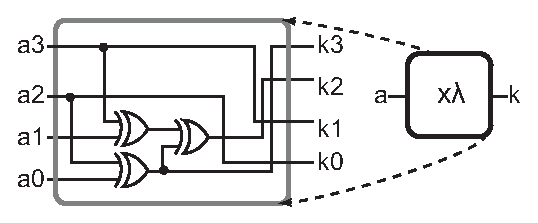
\includegraphics[width=3.2in]{eps/gf24lambda.eps}
  %  \epsfxsize=3.2in
  %  \epsffile{eps/gf24lambda.eps} 

  \caption{
  The illustration reports the implementation logic structure of the \(GF(2^4)\) constant multiplication module.     
  }
  \label{fig:gf24lambda}
  \end{center}
  \vskip -0.2in
\end{figure} 

\begin{table}[t]
 \caption{The pre-calculated  constant \(\lambda\) multiplicative logic verification}
  \label{tab:lambdaGF24}
\centering
%autogenerated by aestest_lambdamultiply via aestest_lambdaGF24.sh
\begin{tabular}{@{\hskip3pt}c@{\hskip3pt}|@{\hskip3pt}c@{\hskip3pt}|@{\hskip3pt}c@{\hskip3pt}|@{\hskip3pt}c@{\hskip3pt}|@{\hskip3pt}c@{\hskip3pt}|@{\hskip3pt}c@{\hskip3pt}|@{\hskip3pt}c@{\hskip3pt}|@{\hskip3pt}c@{\hskip3pt}|@{\hskip3pt}c@{\hskip3pt}|@{\hskip3pt}c@{\hskip3pt}|@{\hskip3pt}c@{\hskip3pt}|@{\hskip3pt}c@{\hskip3pt}|@{\hskip3pt}c@{\hskip3pt}|@{\hskip3pt}c@{\hskip3pt}|@{\hskip3pt}c@{\hskip3pt}|@{\hskip3pt}c@{\hskip3pt}|@{\hskip3pt}c@{\hskip3pt}|}
 \hline
input & 0 & 1 & 2 & 3 & 4 & 5 & 6 & 7 & 8 & 9 & a & b & c & d & e & f \\ 
 \hline
output & 0 & c & 4 & 8 & d & 1 & 9 & 5 & 6 & a & 2 & e & b & 7 & f & 3 \\ 
 \hline
\end{tabular}
\end{table}



\subsection{\(GF(2^4)\) Inversion}
The \(GF(2^4)\) Inversion Module calculates the inversion of the input \(a\), where \(k=a^{-1}\).  The calculated results in reported in Table \ref{tab:invGF24}, and the logic was created by minimizing the Karnaugh Map resulting in

{\renewcommand{\arraystretch}{1.0}%
\begin{align}
\label{equ:invGF24:logicfinal}
%\resizebox{\columnwidth}{!}{
\scalebox{1}{
\( k = \left\{
\begin{array}{ll}
         {k_3}=&a_3 \oplus a_3a_2a_1 \oplus a_3a_0 \oplus a_2 \\
         {k_2}=&a_3a_2a_1 \oplus a_3a_2a_0 \oplus a_3a_0 \oplus a_2 \\
         & \oplus a_2a_1\\
         {k_1}=&a_3\oplus a_3a_2a_1 \oplus a_3a_1a_0 \oplus a_2 \\
          & \oplus a_2a_2 \oplus a_1 \\
         {k_0}=&a_3a_2a_1 \oplus a_3a_2a_0 \oplus a_3a_1\\
           &a_3a_1a_0 \oplus a_3a_0\oplus a_2 \oplus a_2a_1\\
           &a_2a_1a_0 \oplus a_1 \oplus a_0
\end{array}\right.
\)
}
\end{align} 
}
which represents the circuit logic in lieu of a lookup table.  The verification logic for the \(GF(2^4)\) Inversion Module is reported in Table \ref{tab:invGF24}, and this output was automatically generated by the script {aestest\_invGF24.sh}, which iterates through every input.  A single input can be evaluated by 
\begin{lstlisting}[language=bash]
#!/bin/sh
source aesbash.sh
aes_invGF24 "0100"
\end{lstlisting}
where ``0100" in the example above is the binary input of \(a=\{0,1,0,0\}\) resulting in an output of \(k=\{1,1,1,1\}\).

\begin{table}[t]
 \caption{The pre-calculated \(GF(2^4)\) inversion logic verification}
  \label{tab:invGF24}
\centering
%autogenerated by aestest_multinv24 via aestest_multinv24.sh
\begin{tabular}{@{\hskip3pt}c@{\hskip3pt}|@{\hskip3pt}c@{\hskip3pt}|@{\hskip3pt}c@{\hskip3pt}|@{\hskip3pt}c@{\hskip3pt}|@{\hskip3pt}c@{\hskip3pt}|@{\hskip3pt}c@{\hskip3pt}|@{\hskip3pt}c@{\hskip3pt}|@{\hskip3pt}c@{\hskip3pt}|@{\hskip3pt}c@{\hskip3pt}|@{\hskip3pt}c@{\hskip3pt}|@{\hskip3pt}c@{\hskip3pt}|@{\hskip3pt}c@{\hskip3pt}|@{\hskip3pt}c@{\hskip3pt}|@{\hskip3pt}c@{\hskip3pt}|@{\hskip3pt}c@{\hskip3pt}|@{\hskip3pt}c@{\hskip3pt}|@{\hskip3pt}c@{\hskip3pt}|}
 \hline
\(a\) & 0 & 1 & 2 & 3 & 4 & 5 & 6 & 7 & 8 & 9 & a & b & c & d & e & f \\ 
 \hline
\(k^{-1}\) & 0 & 1 & 3 & 2 & f & c & 9 & b & a & 6 & 8 & 7 & 5 & e & d & 4 \\ 
 \hline
\end{tabular}
\end{table}

\section{Conclusion}
The focus of this work was a reference S-Box for AES with a focus on the circuit implementation for the multiplicative inversion module.  The complete mathematical justification has been presented, and is complimented  a BASH script for logic verification that can be used for comparisons against outputs using SPICE.

\section*{Acknowledgment}
This research was supported in part by an appointment to the Intelligence Community Postdoctoral Research Fellowship Program at the Georgia Institute of Technology, administered by Oak Ridge Institute for Science and Education through an interagency agreement between the U.S. Department of Energy and the Office of the Director of National Intelligence.

Brian Degnan would also like thank Ella Rose for her assistance in all things cryptography, Professor Gregory Durgin for his continued support, and Suigin Maeda for general thoughts in the field of mathematics.

%
%\section{AES Key Schedule}
%The key schedule takes the original key derives the subkeys that are used in each round.  The AES key schedule is ``word" orient, where each word is 32-bits.  Words are denoted in the following sections by the term ``\(W\)".  
%
%
%\subsection{128-bit Key Schedule}
%The AES128/128 key schedule has 10 rounds (\(n=10\)), but as the counter starts at \(0\), this gives a total of \(11\) subkeys.  This gives a total of 44 key word elements from \(W\left[0\right]-W\left[43\right]\).  It is worth noting that the original key is the first subkey.  The architecture of the key expansion for encryption is shown in Figure \ref{fig:aes-keyschedule}.  The function \(g()\) is a non-linear function that rotates the input word, performs an S-Box substitution, and adds a round constant (rcon) based on the round number, \(i\).
%\begin{figure}[t]
%  \begin{center}
%  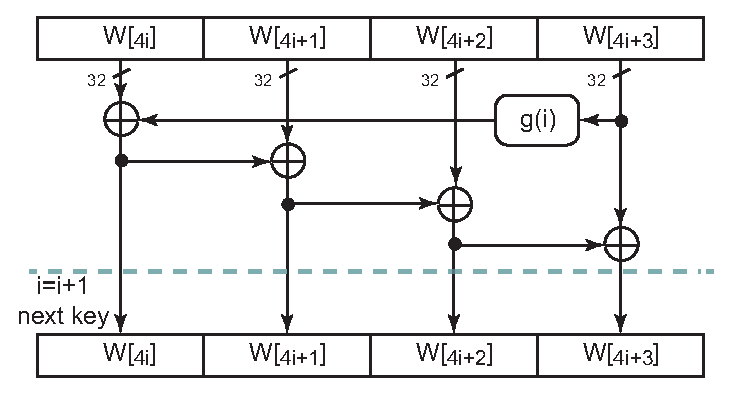
\includegraphics[width=3.0in]{eps/aes-keyschedule.eps}
%  \caption{
%  The illustration describes the logic used for the key expansion during encryption for AES 128/128.  In the illustration, the value \(i\) is the round counter that starts at \(0\) and ends at \(10\).  The function \(g(i)\) is a non-linear function that only operates on the lowest index word.  
%  }
%  \label{fig:aes-keyschedule}
%  \end{center}
%  \vskip -0.2in
%\end{figure} 
%
%
%\subsection{Round Constant}
%\label{ssec:roundconstant}
%The roundconstant module calculates the rcon value needed for the key expansion.  A single input can be evaluated by
%\begin{lstlisting}[language=bash]
%#!/bin/sh
%source aesbash.sh
%aes_roundconstant "01001101" "0"
%\end{lstlisting}
%where ``01001101" is the value for round 13, and ``0" makes the function count in an ascending order. The resulting output is ``10011010".  Changing the second argument to be a ``1" makes the round counter descend, which is used in decryption.   
%
%
%\subsection{RotWord}
%\label{ssec:rotword}
%The RotWord Module calculates an 8-bit left roll of a 32-bit word.
%
%\begin{lstlisting}[language=bash]
%#!/bin/sh
%source aesbash.sh
%data=$(bashUTILhex2bin "0000000f")
%data=$(aes_RotWord $data)
%data=$(bashUTILbin2hex $data)
%echo "$data"
%\end{lstlisting}
%where ``0000000f" in the example above is the value of the 32-bit word to be rotated.  The result is ``00000f00".
%\section{Semiconductor Implementation}
%
\bibliographystyle{IEEEtran}
\bibliography{aesreferences}
% that's all folks
\end{document}


